% Converted from reference/DB4OFlare (MadCap Flare, Java target)

\chapter{Advanced Features}
\label{ref:advanced-topics}

This topic is about advanced features of db4o.

If you want to have multiple unit of work or multiple transaction in embedded mode you can take a look at session containers. \hyperref[ref:advanced-topics-session-containers]{See "Session Containers"} (p.~\pageref{ref:advanced-topics-session-containers})

db4o support unique constrains on fields. \hyperref[ref:advanced-topics-unique-constraints]{See "Unique Constraints"} (p.~\pageref{ref:advanced-topics-unique-constraints})

You can also do backups of your database at runtime. \hyperref[ref:advanced-topics-backup]{See "Backup"} (p.~\pageref{ref:advanced-topics-backup})

Implementing the interfaces for transparent activation/persistence is tedious. The enhancement tools can do that job for you. And can also optimize native queries at build time. \hyperref[ref:advanced-topics-enhancement-tools]{See "Enhancement Tools"} (p.~\pageref{ref:advanced-topics-enhancement-tools})

The database file can fragment over time. In order to reclaim defragmentet space in the database you need to run the defragmentation. \hyperref[ref:advanced-topics-defragment]{See "Defragment"} (p.~\pageref{ref:advanced-topics-defragment})

Callbacks allow you to perform additional logic for different database operations. \hyperref[ref:advanced-topics-callbacks]{See "Callbacks"} (p.~\pageref{ref:advanced-topics-callbacks})

As some point in time you will change your data model. Then you probably need to also refactor you're stored data in the database. \hyperref[ref:advanced-topics-refactoring-and-schema-evolution]{See "Refactoring and Schema Evolution"} (p.~\pageref{ref:advanced-topics-refactoring-and-schema-evolution})

You can access the internal ids or generate UUIDs for objects. \hyperref[ref:advanced-topics-ids-and-uuids]{See "IDs and UUIDs"} (p.~\pageref{ref:advanced-topics-ids-and-uuids})

It's also possible to access the meta information of all stored types in the database. \hyperref[ref:advanced-topics-db4o-meta-information]{See "db4o Meta-Information"} (p.~\pageref{ref:advanced-topics-db4o-meta-information}). And you can access system information about the database.

db4o tried hard to make persisting objects as easy as possible. However storing a object efficient and correctly is quite tricky. Read about db4o's type handling for more information. \hyperref[ref:advanced-topics-type-handling]{See "Type Handling"} (p.~\pageref{ref:advanced-topics-type-handling}) Furthermore db4o uses an abstraction layer to encapsulate Java-reflection. This allows you do change how reflection behaves on your objects. \hyperref[ref:advanced-topics-db4o-reflection-api]{See "db4o Reflection API"} (p.~\pageref{ref:advanced-topics-db4o-reflection-api})

Unfortunately failure happen. db4o communicates failures with exceptions. \hyperref[ref:advanced-topics-exceptions]{See "Exception-Handling"} (p.~\pageref{ref:advanced-topics-exceptions})

\section{Session Containers}
\label{ref:advanced-topics-session-containers}

In an application there are often multiple operations running at the same time. A typical example is a web application which processes multiple requests at the same time. These operations should be isolated from each other. This means that for the database we want to have multiple transactions at the same time. Each transaction does some work and other transactions shouldn't interfere .

db4o supports this scenario with session containers. A session container is a lightweight object-container with its own transaction and reference cache, but shares the resources with its parent container. That means you can commit and rollback changes on such a session container without disturbing the work of other session containers. If you want to implement units of work, you might considers using a session container for each unit. You can create such a container with the open session call.

\begin{lstlisting}
ObjectContainer rootContainer = Db4oEmbedded.openFile(DATABASE_FILE_NAME);

// open the db4o-session. For example at the beginning for a web-request
ObjectContainer session = rootContainer.ext().openSession();
try {
    // do the operations on the session-container
    session.store(new Person("Joe"));
} finally {
    // close the container. For example when the request ends
    session.close();
}
\end{lstlisting}

{\small\itshape Db4oSessions.java: Session object container\par}
\medskip

\subsection*{Transactions And Isolation}

As previously mentioned session-containers are isolated from each other. Each session container has its own transaction and its own reference system. This isolation ensures that the different session container don't interfere witch each other.

They don't share the objects loaded and stored with each other. That means you need to load and store the a object with the same session container. When you try to load a object form one session-container and store it with another, you well end up with two separate copies of that object.

Since the transactions are isolated, changes are only visible for other session containers when you've committed. Before the commit call the changes are not visible to other session containers.

\begin{lstlisting}
session1.store(new Person("Joe"));
session1.store(new Person("Joanna"));

// the second session won't see the changes until the changes are committed
printAll(session2.query(Person.class));

session1.commit();

// new the changes are visiable for the second session
printAll(session2.query(Person.class));
\end{lstlisting}

{\small\itshape Db4oSessions.java: Session are isolated from each other\par}
\medskip

Note also that sessions also have their own reference cache. So when a object is already loaded, it wont be refreshed if another transaction updates the object. You explicitly need to refresh it.

\begin{lstlisting}
Person personOnSession1 = session1.query(Person.class).get(0);
Person personOnSession2 = session2.query(Person.class).get(0);

personOnSession1.setName("NewName");
session1.store(personOnSession1);
session1.commit();

// the second session still sees the old value, because it was cached
System.out.println(personOnSession2.getName());
// you can explicitly refresh it
session2.ext().refresh(personOnSession2, Integer.MAX_VALUE);
System.out.println(personOnSession2.getName());
\end{lstlisting}

{\small\itshape Db4oSessions.java: Each session does cache the objects\par}
\medskip

\section{Unique Constraints}
\label{ref:advanced-topics-unique-constraints}

Unique constraints allow a user to define a field to be unique across all the objects of a particular class stored to db4o. This means that you cannot save an object where a previously committed object has the same field value for fields marked as unique. A Unique Constraint is checked at commit-time and a constraint violation will cause a UniqueFieldValueConstraintViolationException to be thrown. This functionality is based on \hyperref[ref:advanced-topics-callbacks-commit-time-callbacks]{Commit-Time Callbacks} (p.~\pageref{ref:advanced-topics-callbacks-commit-time-callbacks}) feature.

\subsection*{How To Use Unique Constraints}

First you need to add an index on the field which should be unique. After that you add the UniqueFieldValueConstraint to the configuration for the unique field.

\begin{lstlisting}
config.common().objectClass(UniqueId.class).objectField("id").indexed(true);
config.common().add(new UniqueFieldValueConstraint(UniqueId.class, "id"));
\end{lstlisting}

{\small\itshape UniqueConstrainExample.java: Add the index the field and then the unique constrain\par}
\medskip

After that, the unique constrain is applied. When you commit a transaction the uniqueness of the field is checked. If there's any violation, the UniqueFieldValueConstraintViolationException will be thrown.

\begin{lstlisting}
container.store(new UniqueId(42));
container.store(new UniqueId(42));
try {
    container.commit();
} catch (UniqueFieldValueConstraintViolationException e) {
    e.printStackTrace();
}
\end{lstlisting}

{\small\itshape UniqueConstrainExample.java: Violating the constrain throws an exception\par}
\medskip

\subsection*{Client-Server}

In client server mode you need to configure the unique constrains on the server side.

\section{Backup}
\label{ref:advanced-topics-backup}

db4o supplies hot backup functionality to backup single-user databases and client-server databases while they are running.

\begin{lstlisting}
container.ext().backup("backup.db4o");
\end{lstlisting}

{\small\itshape BackupExample.java: Store a backup while using the database\par}
\medskip

Maybe you want to use a other storage system for the backup than the main database. You can specify the storage system for the backup directly:

\begin{lstlisting}
container.ext().backup(new FileStorage(),"advanced-backup.db4o");
\end{lstlisting}

{\small\itshape BackupExample.java: Store a backup with storage\par}
\medskip

The methods can be called while an object container is open and they will execute with low priority in a dedicated thread, with as little impact on processing performance as possible. All concurrent changes to the database will be applied to the backup as well. This process will usually take significantly longer than a plain file copy.

To perform a faster backup that blocks all concurrent database activity, use \textbf{backupSync} instead.

\section{IDs And UUIDs}
\label{ref:advanced-topics-ids-and-uuids}

The db4o team recommends not to use object IDs where it is not necessary. db4o keeps track of object identities in a transparent way, by identifying "known" objects on updates. \hyperref[ref:basics-identity-concept]{See "Identity Concept".} (p.~\pageref{ref:basics-identity-concept})

If you really need to have ids for you're object, take a look at this comparison. \hyperref[ref:platform-specific-issues-disconnected-objects-comparison-of-ids]{See "Comparison Of Different IDs"} (p.~\pageref{ref:platform-specific-issues-disconnected-objects-comparison-of-ids})

\subsection*{Internal IDs}

Each object, except value objects like ints, floats or string, do have an internal id. This id is unique within on db4o database and db4o uses it internally for managing the objects. However you also can access this id or retrieve objects by the internal id.

You can get the internal id of an object from the extended object container.

\begin{lstlisting}
long interalId = container.ext().getID(obj);
\end{lstlisting}

{\small\itshape Db4oInternalIdExample.java: get the db4o internal ids\par}
\medskip

And you can retrieve an object by the internal id. Note that when you get an object by its internal id that it won't be activated. Therefore you have to explicitly activate the object.

\begin{lstlisting}
long internalId =idForObject;
Object objectForID = container.ext().getByID(internalId);
// getting by id doesn't activate the object
// so you need to do it manually
container.ext().activate(objectForID);
\end{lstlisting}

{\small\itshape Db4oInternalIdExample.java: get an object by db4o internal id\par}
\medskip

\subsection*{db4o UUIDs}

db4o can also generate a UUIDs for each object. The UUIDs main purpose is to enable \hyperref[drs:welcome]{replication} (p.~\pageref{drs:welcome}). By default db4o doesn't assign a UUID to each object. You have to enable this \hyperref[ref:configuration-file-generate-uuids]{globally} (p.~\pageref{ref:configuration-file-generate-uuids}) or for \hyperref[ref:configuration-objectclass-generate-uuid]{certain types} (p.~\pageref{ref:configuration-objectclass-generate-uuid}). For example:

\begin{lstlisting}
EmbeddedConfiguration configuration = Db4oEmbedded.newConfiguration();
configuration.file().generateUUIDs(ConfigScope.GLOBALLY);
\end{lstlisting}

{\small\itshape FileConfiguration.java: Enable db4o uuids globally\par}
\medskip

A db4o UUID consists of two parts. The first part is the database signature which is unique to the database.

The second part a unique id within the object-container for the object. Both parts together represent a unique id.

You can get the db4o uuid from the extended object container.

\begin{lstlisting}
Db4oUUID uuid = container.ext().getObjectInfo(obj).getUUID();
\end{lstlisting}

{\small\itshape Db4oUuidExample.java: get the db4o-uuid\par}
\medskip

And you can get an object by its UUID. Note that when you get an object by its UUIDthat it won't be activated. Therefore you have to explicitly activate the object.

\begin{lstlisting}
Object objectForId = container.ext().getByUUID(idForObject);
// getting by uuid doesn't activate the object
// so you need to do it manually
container.ext().activate(objectForId);
\end{lstlisting}

{\small\itshape Db4oUuidExample.java: get an object by a db4o-uuid\par}
\medskip

\section{db4o Meta-Information}
\label{ref:advanced-topics-db4o-meta-information}

Db4o meta information API provides an access to the actual structure of db4o database file. Its primary use is \hyperref[ref:advanced-topics-refactoring-and-schema-evolution]{refactoring} (p.~\pageref{ref:advanced-topics-refactoring-and-schema-evolution}).

You can access the meta information via extended object container. You can ask the object container for all stored classes or for a specific class. To find the meta information for a specific class you can provide the full name, the class itself or an instance of a particular type.

Note that db4o also returns information about internal db4o instances which have been stored.

\begin{lstlisting}
// Get the information about all stored classes.
StoredClass[] classesInDB = container.ext().storedClasses();
for (StoredClass storedClass : classesInDB) {
    System.out.println(storedClass.getName());
}

// Information for a certain class
StoredClass metaInfo = container.ext().storedClass(Person.class);
\end{lstlisting}

{\small\itshape MetaInfoExample.java: All stored classes\par}
\medskip

The stored class interface provides all meta information db4o knows about. You can get the name of the class, ask for the instance count, ask for a list of the ids and get the meta info for super classes.

The most important information about the stored classes meta info is the list of the field which are stored. You can get a list of all fields or ask for specific fields. Note that the meta information might return information for fields which don't exist anymore. This is \hyperref[ref:advanced-topics-refactoring-and-schema-evolution-field-type-change]{useful for refactoring} (p.~\pageref{ref:advanced-topics-refactoring-and-schema-evolution-field-type-change}).

\begin{lstlisting}
StoredClass metaInfoForPerson = container.ext().storedClass(Person.class);
// Access all existing fields
for (StoredField field : metaInfoForPerson.getStoredFields()) {
    System.out.println("Field: "+field.getName());
}
// Accessing the field 'name' of any type.
StoredField nameField = metaInfoForPerson.storedField("name", null);
// Accessing the string field 'name'. Important if this field had another time in previous
// versions of the class model
StoredField ageField = metaInfoForPerson.storedField("age",int.class);

// Check if the field is indexed
boolean isAgeFieldIndexed = ageField.hasIndex();

// Get the type of the field
String fieldType = ageField.getStoredType().getName();
\end{lstlisting}

{\small\itshape MetaInfoExample.java: Accessing stored fields\par}
\medskip

On a the field meta information you can find out the name, type and if the field has an index. And you also can access the values of a object via the stored field. This allows you to access information which is stored in the database but has been removed from the class model. This is \hyperref[ref:advanced-topics-refactoring-and-schema-evolution-field-type-change]{useful for refactoring} (p.~\pageref{ref:advanced-topics-refactoring-and-schema-evolution-field-type-change}).

\begin{lstlisting}
StoredClass metaForPerson = container.ext().storedClass(Person.class);
StoredField metaNameField = metaForPerson.storedField("name", null);

ObjectSet<Person> persons = container.query(Person.class);
for (Person person : persons) {
    String name = (String)metaNameField.get(person);
    System.out.println("Name is "+name);
}
\end{lstlisting}

{\small\itshape MetaInfoExample.java: Access via meta data\par}
\medskip

\section{Consistency Check and File Statistics}
\label{ref:advanced-topics-consistency-check}

Both, the consistency check and the file statistics are part of the db4o-X.XX-optional-java5 jar-file. To run the tool you need to have it and the core jar in the class-path. As alternative use the db4o-X.XX-all-java5 jar, which contains all dependencies.

\subsection*{Consistency Check}

To run consistency checks use the com.db4o.consistency.ConsistencyChecker class, like this:

\begin{lstlisting}
java -cp db4oX-X.XX-all-java5.jar com.db4o.consistency.ConsistencyChecker databaseFile.db4o
\end{lstlisting}

This consistency check doesn't check the content of objects. It only checks if the overall structure of the database file is still intact. Also it doesn't offer any repair functionality. It only tells you if the file is corrupted or not.

\subsection*{File Statistics}

To run consistency checks use the com.db4o.filestats.FileUsageStatsCollector class, like this:

\begin{lstlisting}
java -cp db4oX-X.XX-all-java5.jar com.db4o.filestats.FileUsageStatsCollector databaseFile.db4o
\end{lstlisting}

The file statistics return the space usage of objects, indexes etc in bytes. It also returns the statistics for internal objects, managed by db4o.

\section{System Info}
\label{ref:advanced-topics-system-info}

You can ask the object container for basic system information. Following information can be accessed:

\subsection*{Freespace Size}

\begin{lstlisting}
long freeSpaceSize = container.ext().systemInfo().freespaceSize();
System.out.println("Freespace in bytes: "+freeSpaceSize);
\end{lstlisting}

{\small\itshape SystemInfoExamples.java: Freespace size info\par}
\medskip

Returns the freespace size in the database in bytes. When db4o stores modified objects, it allocates a new slot for it. During commit the old slot is freed. Free slots are collected in the freespace manager, so they can be reused for other objects.

This method returns a sum of the size of all free slots in the database file.

To reclaim freespace run \hyperref[ref:advanced-topics-defragment]{Defragment} (p.~\pageref{ref:advanced-topics-defragment}).

\subsection*{Freespace Entry Count}

\begin{lstlisting}
int freeSpaceEntries = container.ext().systemInfo().freespaceEntryCount();
System.out.println("Freespace-entries count: "+freeSpaceEntries);
\end{lstlisting}

{\small\itshape SystemInfoExamples.java: Freespace entry count info\par}
\medskip

Returns the number of entries in the Freespace Manager.A high value for the number of freespace entries is an indication that the database is fragmented and that \hyperref[ref:advanced-topics-defragment]{Defragment} (p.~\pageref{ref:advanced-topics-defragment}) should be run.

\subsection*{Total Size}

\begin{lstlisting}
long databaseSize = container.ext().systemInfo().totalSize();
System.out.println("Database size: "+databaseSize);
\end{lstlisting}

{\small\itshape SystemInfoExamples.java: Database size info\par}
\medskip

Returns the total size of the database on disk.

\section{Concurrency and db4o}
\label{ref:advanced-topics-concurrency}

How should you deal with concurrent access to a db4o database? This chapter gives an overview and guidelines for dealing with that.

\subsection*{Do Not Share an Object Containers Across Threads}

There are some basic rules which you should never break, otherwise strange effects due to race-condition can happen:

\textbf{Never share an object-container instance across threads}, nor share the data-objects across threads. That will almost certainly create race-conditions. The reason is that when you change objects, while other threads read them, you will get inconsistent views on the state of your data model.

Now how do you deal with concurrent operations? Well you need to use some kind of synchronization strategy.

\subsection*{Use an Object Containers per Unit of Work}

You can avoid synchronization when you are using multiple object containers for different units of work. However you need to be aware to the \hyperref[ref:basics-acid-and-transactions-isolation]{isolation level} (p.~\pageref{ref:basics-acid-and-transactions-isolation}) db4o guarantees. \hyperref[ref:advanced-topics-concurrency-object-container-per-unit-of-work]{See "Object Container per Unit of Work"} (p.~\pageref{ref:advanced-topics-concurrency-object-container-per-unit-of-work})

This is often used in web applications, where you have an object container per request.

\subsection*{Sharing an Object Container}

In a desktop/mobile application you usually want to have one consistent view on your data model. Therefore it makes sense to use the same object container in the whole application. That ensures that we always get the same objects throughout the whole application. As long as you don't load of work to different threads, everything is fine.

However as soon as you start to do manipulations on the data model in different threads you need to synchronize these operations. \hyperref[ref:advanced-topics-concurrency-share-object-container-threads]{See "Share a Object Container Across Threads"} (p.~\pageref{ref:advanced-topics-concurrency-share-object-container-threads})

\subsection{Sharing an Object Container Across Threads}
\label{ref:advanced-topics-concurrency-share-object-container-threads}

You want to share an object container across different threads? Then you automatically also share the stored objects across threads, due to the \hyperref[ref:basics-indentity-concept-reference-cache]{reference-cache} (p.~\pageref{ref:basics-indentity-concept-reference-cache}). Therefore you need to synchronize the access to your object-model.

The basic access-pattern should be like this:

\begin{enumerate}
\item Access the lock which protects the data model.
\item Do manipulations on the data model, which may involve operations on the object container.
\item Release the lock.
\end{enumerate}

\subsubsection{Example}
\label{ref:advanced-topics-concurrency-share-object-container-threads:example}

For example we want to do some back-ground updates, while the rest of the application carries on. As soon as we have this kind pattern we need to protect the access to the data model.

For example this operation starts a background task and carries on doing other things:

\begin{lstlisting}
// Schedule back-ground tasks
final Future<?> task = executor.submit(new Runnable() {
    @Override
    public void run() {
        updateSomePeople(container);
    }
});
// While doing other work
listAllPeople(container);
\end{lstlisting}

{\small\itshape LockingOperations.java: Schedule back-ground tasks\par}
\medskip

Unfortunately these two tasks do work on the same data model, which can lead to race conditions. Therefore access to the data model has to be protected.

\begin{lstlisting}
private void updateSomePeople(ObjectContainer container) {
    synchronized (dataLock) {
        final ObjectSet<Person> people = container.query(new Predicate<Person>() {
            @Override
            public boolean match(Person person) {
                return person.getName().equals("Joe");
            }
        });
        for (Person joe : people) {
            joe.setName("New Joe");
            container.store(joe);
        }
    }
}
\end{lstlisting}

{\small\itshape LockingOperations.java: Grab the lock protecting the data\par}
\medskip

\begin{lstlisting}
private void listAllPeople(ObjectContainer container) {
    synchronized (dataLock) {
        for (Person person : container.query(Person.class)) {
            System.out.println(person.getName());
        }
    }
}
\end{lstlisting}

{\small\itshape LockingOperations.java: Grab the lock to show the data\par}
\medskip

\subsubsection{Improving the Locking}
\label{ref:advanced-topics-concurrency-share-object-container-threads:improving}

Of course the locking showed above is very course grained. A simple improvement would be to use \hyperref[ref:advanced-topics-concurrency-read-write-lock-example]{read-write locks} (p.~\pageref{ref:advanced-topics-concurrency-read-write-lock-example}). In the end you need to adapt the locking strategy to your application.

\subsubsection{Creating a Transaction Model}
\label{ref:advanced-topics-concurrency-share-object-container-threads:transactionmodel}

One model which works good for this scenario is to create a transaction abstraction to do your operations on the data model. Then you do all operations in such a transaction. The transaction manages the lock and the db4o transaction. Such an implementation could look like this:

\begin{lstlisting}
public <T> T inTransaction(TransactionFunction<T> transactionClosure) {
    synchronized (lock) {
        try {
            return transactionClosure.inTransaction(database);
        } catch (Exception e) {
            database.rollback();
            throw new TransactionFailedException(e.getMessage(), e);
        } finally {
            database.commit();
        }
    }
}
\end{lstlisting}

{\small\itshape DatabaseSupport.java: A transaction method\par}
\medskip

And then we can use this transaction method when accessing our data model.

\begin{lstlisting}
private void listAllPeople(DatabaseSupport dbSupport) {
    dbSupport.inTransaction(new TransactionAction() {
        @Override
        public void inTransaction(ObjectContainer container) {
            final ObjectSet<Person> result = container.query(Person.class);
            for (Person person : result) {
                System.out.println(person.getName());
            }
        }
    });
}
\end{lstlisting}

{\small\itshape TransactionOperations.java: Use transaction for reading objects\par}
\medskip

\begin{lstlisting}
private void updateAllJoes(DatabaseSupport dbSupport) {
    dbSupport.inTransaction(new TransactionAction() {
        @Override
        public void inTransaction(ObjectContainer container) {
            final ObjectSet<Person> allJoes = container.query(new Predicate<Person>() {
                @Override
                public boolean match(Person person) {
                    return person.getName().equals("Joe");
                }
            });
            for (Person joe : allJoes) {
                joe.setName("New Joe");
                container.store(joe);
            }
        }
    });
}
\end{lstlisting}

{\small\itshape TransactionOperations.java: Use transaction to update objects\par}
\medskip

Remember that this is only an example. You can use other techniques like annotations or aspects to implement the right behavior. And you also can use more sophisticated locks, like \hyperref[ref:advanced-topics-concurrency-read-write-lock-example]{read write locks} (p.~\pageref{ref:advanced-topics-concurrency-read-write-lock-example}). The only thing which is important is that you synchronize the access your shared data objects.

\subsubsection*{Alternatives}

Alternatively you can avoid sharing data objects and rather use multiple object container to manage concurrent data access.

\paragraph{Read Write Lock Example}
\label{ref:advanced-topics-concurrency-read-write-lock-example}

This example is the same as used in the \hyperref[ref:advanced-topics-concurrency-share-object-container-threads]{shared container topic} (p.~\pageref{ref:advanced-topics-concurrency-share-object-container-threads}). Except that it is using read and write locks.

We replace the lock object with a read write lock:

\begin{lstlisting}
private final ReadWriteLock dataLock = new ReentrantReadWriteLock();
\end{lstlisting}

{\small\itshape ReadWriteLockingOperations.java: Read write lock\par}
\medskip

And then on reading operations you use the read lock:

\begin{lstlisting}
private void listAllPeople(ObjectContainer container) {
    dataLock.readLock().lock();
    try{
        for (Person person : container.query(Person.class)) {
            System.out.println(person.getName());
        }

    } finally{
        dataLock.readLock().unlock();
    }
}
\end{lstlisting}

{\small\itshape ReadWriteLockingOperations.java: Grab the read-lock to show the data\par}
\medskip

On insert and update operations you grab the write lock. Note that you need the write lock every time you change some data.

\begin{lstlisting}
private void updateSomePeople(ObjectContainer container) {
    dataLock.writeLock().lock();
    try {
        final ObjectSet<Person> people = container.query(new Predicate<Person>() {
            @Override
            public boolean match(Person person) {
                return person.getName().equals("Joe");
            }
        });
        for (Person joe : people) {
            joe.setName("New Joe");
            container.store(joe);
        }
    } finally {
        dataLock.writeLock().unlock();
    }
}
\end{lstlisting}

{\small\itshape ReadWriteLockingOperations.java: Grab the write-lock to change the data\par}
\medskip

\subparagraph{Read Write Transaction Example}
\label{ref:advanced-topics-concurrency-read-write-lock-example:read}

You can use read write locks also in a transaction abstraction. This example is an extension of \hyperref[ref:advanced-topics-concurrency-share-object-container-threads]{transaction abstraction example} (p.~\pageref{ref:advanced-topics-concurrency-share-object-container-threads}) but with read write locks.

First we introduce the read write lock.

\begin{lstlisting}
private final ReadWriteLock dataLock = new ReentrantReadWriteLock();
\end{lstlisting}

{\small\itshape DatabaseSupportWithReadWriteLock.java: Read write lock\par}
\medskip

Then we implement read and write transaction methods:

\begin{lstlisting}
public <T> T inReadTransaction(TransactionFunction<T> transactionClosure) {
    return inTransaction(dataLock.readLock(),transactionClosure);
}
\end{lstlisting}

{\small\itshape DatabaseSupportWithReadWriteLock.java: The read transaction method\par}
\medskip

\begin{lstlisting}
public <T> T inWriteTransaction(TransactionFunction<T> transactionClosure) {
    return inTransaction(dataLock.writeLock(),transactionClosure);
}
\end{lstlisting}

{\small\itshape DatabaseSupportWithReadWriteLock.java: The write transaction method\par}
\medskip

\begin{lstlisting}
private <T> T inTransaction(Lock lockToGrab,TransactionFunction<T> transactionClosure) {
    lockToGrab.lock();
    try {
        return transactionClosure.inTransaction(database);
    } catch (Exception e) {
        database.rollback();
        throw new TransactionFailedException(e.getMessage(), e);
    } finally {
        database.commit();
        lockToGrab.unlock();
    }
}
\end{lstlisting}

{\small\itshape DatabaseSupportWithReadWriteLock.java: The transaction implementation\par}
\medskip

After that we can use these operations in our code:

\begin{lstlisting}
private void listAllPeople(DatabaseSupportWithReadWriteLock dbSupport) {
    dbSupport.inReadTransaction(new TransactionAction() {
        @Override
        public void inTransaction(ObjectContainer container) {
            final ObjectSet<Person> result = container.query(Person.class);
            for (Person person : result) {
                System.out.println(person.getName());
            }
        }
    });
}
\end{lstlisting}

{\small\itshape ReadWriteTransactionOperations.java: Use a read transaction for reading objects\par}
\medskip

\begin{lstlisting}
private void updateAllJoes(DatabaseSupportWithReadWriteLock dbSupport) {
    dbSupport.inWriteTransaction(new TransactionAction() {
        @Override
        public void inTransaction(ObjectContainer container) {
            final ObjectSet<Person> allJoes = container.query(new Predicate<Person>() {
                @Override
                public boolean match(Person person) {
                    return person.getName().equals("Joe");
                }
            });
            for (Person joe : allJoes) {
                joe.setName("New Joe");
                container.store(joe);
            }
        }
    });
}
\end{lstlisting}

{\small\itshape ReadWriteTransactionOperations.java: Use a write transaction to update objects\par}
\medskip

\subsection{Object Container per Unit of Work}
\label{ref:advanced-topics-concurrency-object-container-per-unit-of-work}

One possibility is to use an object container per unit of work and avoid sharing it across threads. A typical example is to use an object container per request. You can create a new \hyperref[ref:advanced-topics-session-containers]{session object container at any time} (p.~\pageref{ref:advanced-topics-session-containers}).

Let's take a look at an example. This operation starts a background task and carries on doing other things:

\begin{lstlisting}
// Schedule back-ground tasks
final Future<?> task = executor.submit(new Runnable() {
    @Override
    public void run() {
        updateSomePeople(container);
    }
});
// While doing other work
listAllPeople(container);
\end{lstlisting}

{\small\itshape UnitsOfWork.java: Schedule back-ground tasks\par}
\medskip

In this example we use an object container for the background work:

\begin{lstlisting}
private void updateSomePeople(ObjectContainer rootContainer) {
    ObjectContainer container = rootContainer.ext().openSession();
    try {
        final ObjectSet<Person> people = container.query(new Predicate<Person>() {
            @Override
            public boolean match(Person person) {
                return person.getName().equals("Joe");
            }
        });
        for (Person joe : people) {
            joe.setName("New Joe");
            container.store(joe);
        }
    } finally {
        container.close();
    }
}
\end{lstlisting}

{\small\itshape UnitsOfWork.java: An object container for the background task\par}
\medskip

And another background container for the list task.

\begin{lstlisting}
private void listAllPeople(ObjectContainer rootContainer) {
    ObjectContainer container = rootContainer.ext().openSession();
    try {
        for (Person person : container.query(Person.class)) {
            System.out.println(person.getName());
        }
    } finally {
        container.close();
    }
}
\end{lstlisting}

{\small\itshape UnitsOfWork.java: An object container for this unit of work\par}
\medskip

\subsubsection*{Be Aware of the Isolation Level}

When using multiple object containers you need to be aware of the \hyperref[ref:basics-acid-and-transactions-isolation]{transaction isolation} (p.~\pageref{ref:basics-acid-and-transactions-isolation}). db4o has read committed isolation properties. This isolation applies per object level. Object are loaded individually, which means that the different object-states may are from different committed states.

Here's an example to demonstrate the isolation level issues. We have two bank accounts. One transaction lists the two bank accounts and sums up the total.

\begin{lstlisting}
long moneyInOurAccounts = 0;
List<BankAccount> bankAccounts = container.query(BankAccount.class);
for (BankAccount account : bankAccounts) {
    System.out.println("This account has "+account.money());
    moneyInOurAccounts +=account.money();
    moveMoneyTransactionFinishes();
}
// We get the wrong answer here
System.out.println("The money total is "+moneyInOurAccounts
        +". Expected is "+INITIAL_MONEY_ON_ONE_ACCOUNT*bankAccounts.size());
\end{lstlisting}

{\small\itshape InconsistentStateRead.java: We list the bank accounts and sum up the money\par}
\medskip

During that operation another transaction finishes a money transfer from one account to another and commits.

\begin{lstlisting}
List<BankAccount> bankAccounts = container.query(BankAccount.class);
final BankAccount debitAccount = bankAccounts.get(0);
final BankAccount creditAccount = bankAccounts.get(1);

int moneyToTransfer = 200;
creditAccount.withdraw(moneyToTransfer);
debitAccount.deposit(moneyToTransfer);

container.store(debitAccount);
container.store(creditAccount);
container.commit();
\end{lstlisting}

{\small\itshape InconsistentStateRead.java: Meanwhile we transfer money.\par}
\medskip

Now the other transaction sees one bank account previous transfer, the other account is in the last committed state. Therefore it sees an inconsistent view across these two objects.

\section{Defragment}
\label{ref:advanced-topics-defragment}

A db4o database file is structured as sets of free and occupied slots, similar to a file system. And just like a file system it can be fragmented, resulting in a file that is larger than it needs to be.

The defragmentation API helps to fix this problem. It creates a new database file and copies all objects from the current database file to the new database file. All indexes are recreated. The resulting database file will be smaller and faster. It is recommended to apply defragmentation on a regular basis to achieve better performance.

Take a look how to defragment your database. \hyperref[ref:advanced-topics-defragment-how-to-use-defragmentation]{See "How To Use Defragmentation"} (p.~\pageref{ref:advanced-topics-defragment-how-to-use-defragmentation})

Take a look at the defragmentation configuration options. \hyperref[ref:advanced-topics-defragment-defragmentation-configuration]{See "Defragmentation Configuration"} (p.~\pageref{ref:advanced-topics-defragment-defragmentation-configuration})

You can register a defragmentation listener which notifies you for certain issues: \hyperref[ref:advanced-topics-defragment-tracking-defragmentation-errors]{See "Tracking Defragmentation Errors"} (p.~\pageref{ref:advanced-topics-defragment-tracking-defragmentation-errors})

\subsection{How To Use Defragmentation}
\label{ref:advanced-topics-defragment-how-to-use-defragmentation}

The simplest way to defragment a db4o file would be:

\begin{lstlisting}
Defragment.defrag("database.db4o");
\end{lstlisting}

{\small\itshape DefragmentationExample.java: Simplest possible defragment use case\par}
\medskip

Ensure that the file is not opened by any other process or db4o instance.

This moves the file \emph{filename }to \emph{filename.backup}, then it create a defragmented version of this database at the original position. If the backup file already exists this an IOException is throw and no action will be taken.

You can also specify the backup filename manually:

\begin{lstlisting}
Defragment.defrag("database.db4o", "database.db4o.bak");
\end{lstlisting}

{\small\itshape DefragmentationExample.java: Specify backup file explicitly\par}
\medskip

For more detailed configuration of the defragmentation process, you can use a \hyperref[ref:advanced-topics-defragment-defragmentation-configuration]{DefragmentConfig} (p.~\pageref{ref:advanced-topics-defragment-defragmentation-configuration}) instance:

\begin{lstlisting}
DefragmentConfig config = new DefragmentConfig("database.db4o");
Defragment.defrag(config);
\end{lstlisting}

{\small\itshape DefragmentationExample.java: Defragment with configuration\par}
\medskip

It's possible to use a more fine grained configuration for the deframentation process. \hyperref[ref:advanced-topics-defragment-defragmentation-configuration]{See "Defragmentation Configuration"} (p.~\pageref{ref:advanced-topics-defragment-defragmentation-configuration})

Defragmentation can throw IOException in the following situations:

\begin{itemize}
\item Backup file exists.
\item Database file not found.
\item Database file is opened by another process.
\end{itemize}

\subsection{Defragmentation Configuration}
\label{ref:advanced-topics-defragment-defragmentation-configuration}

You can configure the defragmentation processes for your needs. This topic discusses the available configuration options.

First you need to configure which database file to defragment. \hyperref[ref:advanced-topics-defragment-configuration-database-files]{See "Original Database And Backup"} (p.~\pageref{ref:advanced-topics-defragment-configuration-database-files})

It's also recommended to use the db4o database configuration for the defragmentation process. This ensures that all low level settings which influence the database-file layout are used. \hyperref[ref:advanced-topics-defragment-configuration-database-configuration]{See "Database Configuration"} (p.~\pageref{ref:advanced-topics-defragment-configuration-database-configuration})

When you defragment large database you should configure a commit-frequency to speed up the defragmentation process. \hyperref[ref:advanced-topics-defragment-configuration-commit-frequency]{See "Commit Frequency"} (p.~\pageref{ref:advanced-topics-defragment-configuration-commit-frequency})

If you have refractored your classes you might want to remove old meta data. This is possible with the class filters. \hyperref[ref:advanced-topics-defragment-configuration-class-filter]{See "Class Filter"} (p.~\pageref{ref:advanced-topics-defragment-configuration-class-filter})

By default the backup file isn't deleted after a successful defragmentation. You can change that. \hyperref[ref:advanced-topics-defragment-configuration-delete-backup]{See "Delete The Backup"} (p.~\pageref{ref:advanced-topics-defragment-configuration-delete-backup})

You can force a database update before defragmenting the database-file. \hyperref[ref:advanced-topics-defragment-configuration-upgrade-db]{See "Upgrade Database File"} (p.~\pageref{ref:advanced-topics-defragment-configuration-upgrade-db})

You can disable the read-only more the for backup file. \hyperref[ref:advanced-topics-defragment-configuration-disable-read-only]{See "Disable Read Only Mode"} (p.~\pageref{ref:advanced-topics-defragment-configuration-disable-read-only})

If you want to have different storage implementation for the old database file and the new defragmented database file you can configure a separate storage. \hyperref[ref:advanced-topics-defragment-configuration-storage-backupdb]{See "Configure Storage for Backup File"} (p.~\pageref{ref:advanced-topics-defragment-configuration-storage-backupdb})

You can change the id-mapping implementation for the defragmentation-process. \hyperref[ref:advanced-topics-defragment-configuration-id-mapping]{See "Configure IDMapping"} (p.~\pageref{ref:advanced-topics-defragment-configuration-id-mapping})

\subsubsection{Original Database And Backup}
\label{ref:advanced-topics-defragment-configuration-database-files}

The database-file which needs to be defragmented is specified in the configuration. The first constructor parameter is the database file.

\begin{lstlisting}
DefragmentConfig config = new DefragmentConfig("database.db4o");

Defragment.defrag(config);
\end{lstlisting}

{\small\itshape DefragmentationConfigurationExamples.java: Configure the file\par}
\medskip

The defragmentation process creates a backup of the old database. By default the back-up file has the name of the original database-file with an additional '.backup'-suffix. You can explicitly specify the backup file name with the second constructor parameter.

\begin{lstlisting}
DefragmentConfig config = new DefragmentConfig("database.db4o", "database.db4o.back");

Defragment.defrag(config);
\end{lstlisting}

{\small\itshape DefragmentationConfigurationExamples.java: Configure the file and backup file\par}
\medskip

\subsubsection{Database Configuration}
\label{ref:advanced-topics-defragment-configuration-database-configuration}

Perhaps you're using low level configuration settings which are \hyperref[ref:configuration-file-configuration]{file-related} (p.~\pageref{ref:configuration-file-configuration}). In such cases it's recommended to use the database configuration for the defragmentation process. Especially settings like \hyperref[ref:configuration-common-string-encoding]{string-encoding} (p.~\pageref{ref:configuration-common-string-encoding}) and \hyperref[ref:configuration-file-block-size]{block-size} (p.~\pageref{ref:configuration-file-block-size}) need to be configured properly for the defragmentation.

\begin{lstlisting}
DefragmentConfig config = new DefragmentConfig("database.db4o");
// It's best to use the very same configuration you use for the regular database
final EmbeddedConfiguration configuration = Db4oEmbedded.newConfiguration();
config.db4oConfig(configuration);

Defragment.defrag(config);
\end{lstlisting}

{\small\itshape DefragmentationConfigurationExamples.java: Use the database-configuration\par}
\medskip

\subsubsection{Commit Frequency}
\label{ref:advanced-topics-defragment-configuration-commit-frequency}

The defragmentation system uses db4o's transactional core to write the data to the new defragmented file. For large databases managing a long transaction can become an issue and can slow down the defragmentation. Therefore you can set a commit frequency. This means after the set number of processed objects the transaction is committed on the new file.

\begin{lstlisting}
DefragmentConfig config = new DefragmentConfig("database.db4o");
config.objectCommitFrequency(10000);

Defragment.defrag(config);
\end{lstlisting}

{\small\itshape DefragmentationConfigurationExamples.java: Set the commit frequency\par}
\medskip

\subsubsection{Class Filter}
\label{ref:advanced-topics-defragment-configuration-class-filter}

db4o stores meta data about all classes used in the database . Even when the class doesn't exist anymore the meta-data in db4o is still there. The class filter allows you to remove class-meta data from the defragmented database. You can pass you own implementation of a class filter. Or you can use the built in AvailableClassFilter. This filter removes all meta-data of classes which aren't present anymore.

\begin{lstlisting}
DefragmentConfig config = new DefragmentConfig("database.db4o");
config.storedClassFilter(new AvailableClassFilter());

Defragment.defrag(config);
\end{lstlisting}

{\small\itshape DefragmentationConfigurationExamples.java: Use class filter\par}
\medskip

\subsubsection{Delete The Backup}
\label{ref:advanced-topics-defragment-configuration-delete-backup}

The defragmentation process copies the data from the old database to a new file. The old file is left as a backup. You can force the defragmentation process to delete the backup after a successful defragmenting.

\begin{lstlisting}
DefragmentConfig config = new DefragmentConfig("database.db4o");
config.forceBackupDelete(true);

Defragment.defrag(config);
\end{lstlisting}

{\small\itshape DefragmentationConfigurationExamples.java: Delete the backup after the defragmentation process\par}
\medskip

\subsubsection{Upgrade Database File}
\label{ref:advanced-topics-defragment-configuration-upgrade-db}

This option will upgrade first the database file format and then defragment it. You need to specify a folder where the temporary data for this process is stored.

\begin{lstlisting}
DefragmentConfig config = new DefragmentConfig("database.db4o");
config.upgradeFile(System.getProperty("java.io.tmpdir"));

Defragment.defrag(config);
\end{lstlisting}

{\small\itshape DefragmentationConfigurationExamples.java: Upgrade database version\par}
\medskip

\subsubsection{Disable Read Only Mode}
\label{ref:advanced-topics-defragment-configuration-disable-read-only}

By default the back-up database is opened in read only mode. You can disable the read only mode if you want.

\begin{lstlisting}
DefragmentConfig config = new DefragmentConfig("database.db4o");
config.readOnly(false);

Defragment.defrag(config);
\end{lstlisting}

{\small\itshape DefragmentationConfigurationExamples.java: Disable readonly on backup\par}
\medskip

\subsubsection{Configure Storage for Backup File}
\label{ref:advanced-topics-defragment-configuration-storage-backupdb}

By default the defragmentation process uses the storage from the db4o configuration for both database files, the backup and the new defragmented database file. If you want to have different storage implementations you can specify a different storage for the backup-file. This way the new defragmented database-file uses the storage from the database-configuration and the backup-file uses the back-up storage.

\begin{lstlisting}
DefragmentConfig config = new DefragmentConfig("database.db4o");
config.backupStorage(new FileStorage());

Defragment.defrag(config);
\end{lstlisting}

{\small\itshape DefragmentationConfigurationExamples.java: Use a separate storage for the backup\par}
\medskip

\subsubsection{Configure IDMapping}
\label{ref:advanced-topics-defragment-configuration-id-mapping}

When you defragment a database each object is stored at a new location. To keep track which old id maps the which new location a IDMapper is uses. You can change the IDMapper or even implement your own.

By default the InMemoryIdMapping is uses, which is the fastest version, but consumes the most memory. As alterative there's the DatabaseIdMapping available, which stores mapping in a file and therefore uses less memory.

\begin{lstlisting}
IdMapping mapping = new InMemoryIdMapping();
DefragmentConfig config = new DefragmentConfig("database.db4o", "database.db4o.back", mapping);

Defragment.defrag(config);
\end{lstlisting}

{\small\itshape DefragmentationConfigurationExamples.java: Choose a id mapping system\par}
\medskip

\subsection{Tracking Defragmentation Errors}
\label{ref:advanced-topics-defragment-tracking-defragmentation-errors}

You can pass a defragmentation listener to the defragmentation process. This listener will be notified when there's no object for an id in the database. This means that a object has a reference to a non-existing object. This happens when you delete objects which are still referenced by other objects.

\begin{lstlisting}
DefragmentConfig config = new DefragmentConfig("database.db4o");
Defragment.defrag(config,new DefragmentListener() {
    @Override
    public void notifyDefragmentInfo(DefragmentInfo defragmentInfo) {
        System.out.println(defragmentInfo);
    }
});
\end{lstlisting}

{\small\itshape DefragmentationExample.java: Use a defragmentation listener\par}
\medskip

\section{Enhancement Tools}
\label{ref:advanced-topics-enhancement-tools}

Enhancement tools provide a convenient framework for application (jar, dll, exe) or classes modification to support db4o-specific functionality. Enhancement tools can work on a ready application or library and apply the improvements at load or build time.

The tools functionality is provided through bytecode instrumentation. This process inserts special, usually short, sequences of bytecode at designated points in your code. It is typically used for profiling or monitoring, however the range of use of bytecode instrumentation is not limited by this tasks: it can be applied anywhere where a specific functionality should be plugged into the ready built classes.

db4o Enhancement Tools currently have these cases for bytecode instrumentation:

\begin{itemize}
\item \hyperref[ref:basics-activation-concept-transparent-activation-framework]{Transparent Activation} (p.~\pageref{ref:basics-activation-concept-transparent-activation-framework})
\item \hyperref[ref:basics-update-concept-transparent-persistence]{Transparent Persistence} (p.~\pageref{ref:basics-update-concept-transparent-persistence})
\item \hyperref[ref:basics-querying-native-queries-native-query-optimization]{Native Query Optimization} (p.~\pageref{ref:basics-querying-native-queries-native-query-optimization})
\end{itemize}

In \hyperref[ref:basics-update-concept-transparent-persistence]{transparent activation/persistence case} (p.~\pageref{ref:basics-update-concept-transparent-persistence}), classes are required to implement Activatable interface to support transparent activation. In many cases you don't want to pollute your classes with some additional interface, or even won't be able to do so if you use a third party classes library. That's where bytecode instrumentation comes handy: Activatable interface will be implemented on your existing classes by applying bytecode instrumentation. Another advantage of this approach - you can still work on your "clean" classes, just do not forget to run the instrumentation afterwards.

In the native query optimization case bytecode instrumentation is used as a more performant alternative to a run-time optimization. When an native query is optimized the user and compiler-friendly syntax of NQ predicate is replaced with a query-processor-friendly code. Obviously, optimization process can take some time, therefore it can be a good choice to use pre-instrumented classes, then to let the optimization be executed each time it is required by application.

The instrumentation can be run at build time, also known as static instrumentation. In this case a special build script calls runs the instrumentation on the classes before packaging them to jar, or on the jar itself. This is the fastest solution as no time is spent on bytecode instrumentation at runtime.

Another method is to use bytecode instrumentation at load time. In this case instrumenting information is inserted into the classes by a specific instrumenting classloader just before they are loaded into the VM.

There are different possibilities to integrate the enhancement tools into a project.

\begin{itemize}
\item More details about built time enhancements: \hyperref[ref:advanced-topics-enhancement-tools-enhancement-for-java-build-time-enhancement]{See "Build Time Enhancement"} (p.~\pageref{ref:advanced-topics-enhancement-tools-enhancement-for-java-build-time-enhancement})
\item It's possible to enhance the classes a runtime:
\end{itemize}

\subsection{Enhancement Example}
See section~\ref{ref:basics-transparentpersistence-ta-enhanced-example} on page~\pageref{ref:basics-transparentpersistence-ta-enhanced-example}.

\subsection{Build Time Enhancement}
\label{ref:advanced-topics-enhancement-tools-enhancement-for-java-build-time-enhancement}

You can enhance your classes at build time. The main use for the enhancement process is to add the activate interface implementation to the persisted classes. A load time \hyperref[ref:basics-transparentpersistence-ta-enhanced-example]{enhancement example is available here} (p.~\pageref{ref:basics-transparentpersistence-ta-enhanced-example}).

This topic explains the individual elements of the ant task.

\subsubsection*{Dependencies.}

For transparent activation/persistence you need following dependencies at compile time. (see also the \hyperref[ref:dependency-overview]{dependency overview} (p.~\pageref{ref:dependency-overview}))

\begin{itemize}
\item bloat-1.0.jar
\item db4o-X.XX-instrumentation.jar
\item db4o-X.XX-taj.jar
\item db4o-X.XX-tools.jar
\end{itemize}

\subsubsection*{The Example Script}

This is an example script. Below it each part of it is campaigned and the alternatives to it.

\begin{lstlisting}
<target name="enhance">
    <!-- Change these according to your project -->
    <property name="target" value="./target/classes/"/>
    <property name="libraries" value="./lib/"/>

    <path id="project.classpath">
        <pathelement path="${target}"/>
        <fileset dir="${libraries}">
            <include name="*.jar"/>
        </fileset>
    </path>

    <!-- We enhance with an additional Ant-run step. You can put this also in an extra file -->
    <typedef resource="instrumentation-def.properties"
             classpathref="project.classpath"
             loaderRef="instrumentation.loader"/>

    <!-- We filter by our annotation -->
    <typedef name="annotation-filter"
             classname="com.db4odoc.tp.enhancement.AnnotationFilter"
             classpathref="project.classpath"
             loaderRef="instrumentation.loader"/>

    <db4o-instrument classTargetDir="${target}"
                  verbose="true">
        <classpath refid="project.classpath"/>
        <sources dir="${target}">
            <include name="**/*.class"/>
        </sources>

        <transparent-activation-step>
            <annotation-filter/>
        </transparent-activation-step>
    </db4o-instrument>
</target>
\end{lstlisting}

{\small\itshape enhance-with-annotation.xml: Ant target for enhancing your classes after building them\par}
\medskip

\subsubsection*{The Tags}

{\small
\begin{longtable}{|p{\dimexpr(\linewidth-3\arrayrulewidth)*1/2-2\tabcolsep\relax}|p{\dimexpr(\linewidth-3\arrayrulewidth)*1/2-2\tabcolsep\relax}|}
\hline
\textbf{Tag/Property} & \textbf{Explanation} \\ \hline
property target & Specifies to which classes the enhancement is applied. \\ \hline
property libraries & Specifies where the libraries are. This is used for setting up the classpath of the enhancement step. The enhancement should have access to all classes, otherwise class not found exceptions might occur. \\ \hline
path project.classpath & This represents the whole project classpath: Your code and all libraries. This classpath is passed to the enhancer step. \\ \hline
typedef instrumentation-def.properties & Loads the predefined tasks from the db4o jars. Make sure that all required db4o dependencies are on the classpath. \\ \hline
typedef annotation-filter & This defines a regular Java class as part of the Ant script. This way you can implement your own filter.\par The name attribute specifies how the task is named within the Ant script. \\ \hline
db4o-instrument & The db4o-instrument task, which can do all available instrumentations. In the attribute 'classTargetDir' you specify where to put the enhanced result. \\ \hline
db4o-instrument-\textgreater{}classpath & Here we need to specify the classpath for the enhancer-step. Refer to classpath which includes the application code and the libraries. \\ \hline
db4o-instrument-\textgreater{}sources & Specifies which class-files are enhanced \\ \hline
transparent-activation-step & This tag specifies that the transparent activation/persistence enhancement is applied. This tag expects that you specify one more filters to filter out the classes which need to be enhance.\par For the example filter take a look at \hyperref[ref:basics-transparentpersistence-ta-enhanced-example]{the example} (p.~\pageref{ref:basics-transparentpersistence-ta-enhanced-example}). \\ \hline
native-query-step & You also can specify the native query enhancing step. Usually this is done at runtime, but can be done a compile time. Just add it the the db4o-instrument tag. \\ \hline
\end{longtable}}

\subsubsection*{Simple Enhancer Alternative}

As alternative quick way you can use the 'db4o-enhance'-task. There you just can specify the location of the class files which you want to enhance. It works best when you put all your persistent classes in a separate package or project.

\begin{lstlisting}
<target name="simpleEnhanceStep">
    <db4o-enhance classtargetdir="${basedir}/bin"
                  jartargetdir="../libs/java/"
                  nq="false" ta="true"
                  collections="true"
                  verbose="true">
        <classpath refid="project.classpath"/>
        <sources dir="${basedir}/bin">
                  <include name="com/db4odoc/tp/**/*.class"/>
        </sources>
    </db4o-enhance>
</target>
\end{lstlisting}

{\small\itshape enhance-with-annotation.xml: Simple enhancing step\par}
\medskip

\subsubsection*{Enhancing Classes Using Maven}

As demonstrated \hyperref[ref:basics-transparentpersistence-ta-enhanced-example]{in the example} (p.~\pageref{ref:basics-transparentpersistence-ta-enhanced-example}) you can include a enhancing Ant script in your Maven build. All descriptions above applies. However you can use the built in Maven classpath. Just use the 'maven.compile.classpath' in the Ant script.

\section{Callbacks}
\label{ref:advanced-topics-callbacks}

Callbacks, also known as events, allow you to be notified on certain database operations. This is useful to trigger additional operations during a database operation. There are two kind of callbacks. First you can certain methods to your objects. When the method matches certain signature it will be called by db4o. \hyperref[ref:advanced-topics-callbacks-object-callbacks]{See "Object Callbacks"} (p.~\pageref{ref:advanced-topics-callbacks-object-callbacks})

Additionally you can register event listener to a object-container which will be called on certain operations. \hyperref[ref:advanced-topics-callbacks-event-registry-api]{See "Event Registry API"} (p.~\pageref{ref:advanced-topics-callbacks-event-registry-api})

\subsection{Object Callbacks}
\label{ref:advanced-topics-callbacks-object-callbacks}

Callback methods are automatically called on persistent objects by db4o during certain database events.

For a complete list of the signatures of all available methods see the com.db4o.ext.ObjectCallbacks interface.

You do not have to implement this interface. db4o recognizes the presence of individual methods by their signature, using reflection. You can simply add one or more of the methods to your persistent classes and they will be called.

Returning false to the \texttt{\#objectCanXxxx()} methods will prevent the current action from being taken.

In a client/server environment callback methods will be called on the client with two exceptions:

\texttt{objectOnDelete(), objectCanDelete()}

Some possible usecases for callback methods:

\begin{itemize}
\item Setting default values after refactorings.
\item Checking object integrity before storing objects.
\item Setting transient fields.
\item Restoring connected state (of GUI, files, connections).
\end{itemize}

\subsection{Event Registry API}
\label{ref:advanced-topics-callbacks-event-registry-api}

You can register to events of the db4o-database. You can used these events to implement all kinds of additional functionality. Take a look a few example use-cases. \hyperref[ref:advanced-topics-callbacks-possible-usecases]{See "Possible Usecases"} (p.~\pageref{ref:advanced-topics-callbacks-possible-usecases})

There's an event for each database operation. Most of the time there are two events for an operation. One is fired before the operation starts, the other when the operation ends.

\subsubsection*{Register to an Event}

You can gain access to the events via a event registry. These three steps show how to register to events.

First obtain a EventRegistry-instance from the object container.

\begin{lstlisting}
EventRegistry events = EventRegistryFactory.forObjectContainer(container);
\end{lstlisting}

{\small\itshape EventRegistryExamples.java: Obtain the event-registry\par}
\medskip

Now you can register your event-handlers on the event registry.

\begin{lstlisting}
events.committing().addListener(new EventListener4<CommitEventArgs>() {
    public void onEvent(Event4<CommitEventArgs> source,
                        CommitEventArgs arguments) {
        handleCommitting(source,arguments);
    }
});
\end{lstlisting}

{\small\itshape EventRegistryExamples.java: register for a event\par}
\medskip

Then implement your event handling.

\begin{lstlisting}
private static void handleCommitting(Event4<CommitEventArgs> source,
                                     CommitEventArgs commitEventArgs) {
    // handle the event here
}
\end{lstlisting}

{\small\itshape EventRegistryExamples.java: implement your event handling\par}
\medskip

\subsubsection*{Cancelable Events}

Some events can cancel the operation. All events which have a CancellableObjectEventArgs-parameter can cancel the operation. When you cancel in a event, the operation won't be executed. For example:

\begin{lstlisting}
EventRegistry events = EventRegistryFactory.forObjectContainer(container);
events.creating().addListener(new EventListener4<CancellableObjectEventArgs>() {
    public void onEvent(Event4<CancellableObjectEventArgs> events,
                        CancellableObjectEventArgs eventArgs) {
        if(eventArgs.object() instanceof Person){
            Person p = (Person) eventArgs.object();
            if(p.getName().equals("Joe Junior")){
                eventArgs.cancel();
            }
        }
    }
});
\end{lstlisting}

{\small\itshape EventRegistryExamples.java: Cancel store operation\par}
\medskip

\subsubsection*{Register Events On The Server}

When you want to register for the events on the server, you should register it on the server-container.

\begin{lstlisting}
ObjectServer server = 
        Db4oClientServer.openServer(DATABASE_FILE_NAME, PORT_NUMBER);
EventRegistry eventsOnServer =
        EventRegistryFactory.forObjectContainer(server.ext().objectContainer());
\end{lstlisting}

{\small\itshape EventRegistryExamples.java: register for events on the server\par}
\medskip

\subsubsection*{Commit-Events}

Commit-events bring a collection of the added, updated and deleted object with it. You can iterate over these objects. The updated- and added-collections contain LazyObjectReferences, the deleted-event a FrozenObjectInfos. Note that you may cannot get deleted object-instance anymore, but only the meta-info. Furthermore the object doesn't need to be activated. So when you need to read information out if it, ensure that you've activated it first.

\begin{lstlisting}
EventRegistry events = EventRegistryFactory.forObjectContainer(container);
events.committed().addListener(new EventListener4<CommitEventArgs>() {
    public void onEvent(Event4<CommitEventArgs> events,
                        CommitEventArgs eventArgs) {
        for(Iterator4 it=eventArgs.added().iterator();it.moveNext();){
            LazyObjectReference reference = (LazyObjectReference) it.current();
            System.out.println("Added "+reference.getObject());
        }
        for(Iterator4 it=eventArgs.updated().iterator();it.moveNext();){
            LazyObjectReference reference = (LazyObjectReference) it.current();
            System.out.println("Updated "+reference.getObject());
        }
        for(Iterator4 it=eventArgs.deleted().iterator();it.moveNext();){
            FrozenObjectInfo deletedInfo = (FrozenObjectInfo) it.current();
            // the deleted info might doesn't contain the object anymore and
            // return the null.
            System.out.println("Deleted "+deletedInfo.getObject());
        }
    }
});
\end{lstlisting}

{\small\itshape EventRegistryExamples.java: Commit-info\par}
\medskip

\subsubsection*{Pitfalls and Limitations}

\begin{itemize}
\item All embedded clients-/session share the same event registry. So you need to register the events only on one.
\item You cannot call recursively the event-producing operation within the event-handler. For example in the storing-event you cannot call store. In the committing-event you cannot call commit.
\item In client-server mode, each client has it's own event-registry, and therefore only sees its own events. Except the committed-event. \hyperref[ref:client-server-events-in-cs-mode]{See "Events In Client Server-Mode"} (p.~\pageref{ref:client-server-events-in-cs-mode})
\end{itemize}

\subsection{Events Overview}
\label{ref:advanced-topics-callbacks-events-overview}

This overview shows you all available events. Additionally it shows on which side the event is called in client-server-mode.

{\small
\begin{longtable}{|p{\dimexpr(\linewidth-6\arrayrulewidth)*1/5-2\tabcolsep\relax}|p{\dimexpr(\linewidth-6\arrayrulewidth)*1/5-2\tabcolsep\relax}|p{\dimexpr(\linewidth-6\arrayrulewidth)*1/5-2\tabcolsep\relax}|p{\dimexpr(\linewidth-6\arrayrulewidth)*1/5-2\tabcolsep\relax}|p{\dimexpr(\linewidth-6\arrayrulewidth)*1/5-2\tabcolsep\relax}|}
\hline
\textbf{Event} & \textbf{Explanation} & \textbf{Cancellable} & \textbf{Client} & \textbf{Server} \\ \hline
activating & Fired before a object is activated. & X & X &  \\ \hline
activated & Fired after a object is activated. &  & X &  \\ \hline
creating & Fired before a object is stored to first time. & X & X &  \\ \hline
creating & Fired after a object is stored to first time. &  & X &  \\ \hline
deleting & Fired before a object is deleted. & X &  & X \\ \hline
deleted & Fired after a object is deleted. &  &  & X \\ \hline
updating & Fired before a object is updated. & X & X &  \\ \hline
updated & Fired after a object is updated. &  & X &  \\ \hline
deactivating & Fired before a object is deactivated. & X & X &  \\ \hline
deactivated & Fired after a object is deactivated. & X & X &  \\ \hline
queryStarted & Fired when a query starts. &  & X &  \\ \hline
queryFinished & Fired when a query has finished. &  & X &  \\ \hline
committing & Fired before a commit. &  &  & X \\ \hline
committed & Fired after a commit. &  & X\footnote{This event is asynchronously distributed across all clients} & X \\ \hline
closing & Fired when the object is closed. &  & X &  \\ \hline
classRegistered & Fired when a new class is stored/loaded. &  & X &  \\ \hline
instantiated & Fired when a object is instantiated. &  & X &  \\ \hline
\end{longtable}}

\subsection{Possible Usecases}
\label{ref:advanced-topics-callbacks-possible-usecases}

There are many use cases for external callbacks, including:

\begin{itemize}
\item Cascaded deletes, updates.
\item Referential integrity checks.
\item Gathering statistics.
\item Auto assigned fields .
\item Assigning customary unique IDs for external referencing.
\item Delayed deletion (objects are marked for deletion when delete(object) is called and cleaned out of database in a later maintenance operation).
\item Ensuring object fields uniqueness within the same class etc.
\end{itemize}

More Reading:

\begin{itemize}
\item \hyperref[ref:advanced-topics-callbacks-possible-usecases-referential-integrity]{Referential Integrity} (p.~\pageref{ref:advanced-topics-callbacks-possible-usecases-referential-integrity})
\item \hyperref[ref:advanced-topics-callbacks-possible-usecases-autoincrement]{Autoincrement} (p.~\pageref{ref:advanced-topics-callbacks-possible-usecases-autoincrement})
\end{itemize}

\subsubsection{Autoincrement}
\label{ref:advanced-topics-callbacks-possible-usecases-autoincrement}

db4o does not deliver a field auto increment feature, which is common in RDBMS. Normally you don't need any additional ids, since db4o manages objects by object-identity. However cases where you have \hyperref[ref:platform-specific-issues-disconnected-objects]{disconnected objects} (p.~\pageref{ref:platform-specific-issues-disconnected-objects}), you need additional ids. One of then possibilities it to use auto incremented ids.

If your application logic requires this feature you can implement it using external callbacks. One of the possible solutions is presented below. Note that this example only works in embedded-mode.

This example assumes that all object which need an auto incremented id are subclasses of the IDHolder class. This class contains the auto-incremented id.

\begin{lstlisting}
private int id;
public int getId() {
    return id;
}

public void setId(int id) {
    this.id = id;
}
\end{lstlisting}

{\small\itshape IDHolder.java: id holder\par}
\medskip

First create a class which keeps the state of the auto-increment numbers. For example a map which keeps the latest auto incremented id for each class.

\begin{lstlisting}
private static class PersistedAutoIncrements {
 private final Map<Class, Integer> currentHighestIds = new HashMap<Class, Integer>();

    public int nextNumber(Class forClass) {
        Integer number = currentHighestIds.get(forClass);
        if (null == number) {
            number = 0;
        }
        number += 1;
        currentHighestIds.put(forClass,number);
        return number;
    }
}
\end{lstlisting}

{\small\itshape AutoIncrement.java: persistent auto increment\par}
\medskip

Then create two methods, which are called later. One which returns the next auto-incremented id for a certain class. Another which stores the current state of the auto-increments.

\begin{lstlisting}
public synchronized int getNextID(Class forClass) {
       PersistedAutoIncrements incrementState = ensureLoadedIncrements();
       return incrementState.nextNumber(forClass);
}

   public synchronized void storeState(){
       if(null!=state){
           container.ext().store(state,2);            
       }
   }
\end{lstlisting}

{\small\itshape AutoIncrement.java: getting the next id and storing state\par}
\medskip

The last part is to ensure that the existing auto-increments are loaded from the database. Or if not existing a new instance is created.

\begin{lstlisting}
private PersistedAutoIncrements ensureLoadedIncrements() {
    if(null==state){
        state = loadOrCreateState();
    }
    return state;

}

private PersistedAutoIncrements loadOrCreateState() {
    ObjectSet<PersistedAutoIncrements> existingState = container.query(PersistedAutoIncrements.class);
    if(0==existingState.size()){
        return new PersistedAutoIncrements(); 
    } else if(1==existingState.size()){
        return existingState.get(0);
    } else{
        throw new IllegalStateException("Cannot have more than one state stored in database");
    }
}
\end{lstlisting}

{\small\itshape AutoIncrement.java: load the state from the database\par}
\medskip

Now it's time to use the callbacks. Every time when a new object is created, assign a new id. For this the creating-event is perfect. When commiting also make the auto increment-state persistent, to ensure that no id is used twice.

\begin{lstlisting}
final AutoIncrement increment = new AutoIncrement(container);
EventRegistry eventRegistry = EventRegistryFactory.forObjectContainer(container);
eventRegistry.creating().addListener(new EventListener4<CancellableObjectEventArgs>() {
    public void onEvent(Event4<CancellableObjectEventArgs> event4,
                        CancellableObjectEventArgs objectArgs) {
        if(objectArgs.object() instanceof IDHolder){
            IDHolder idHolder = (IDHolder) objectArgs.object();
            idHolder.setId(increment.getNextID(idHolder.getClass()));
        }
    }
});
eventRegistry.committing().addListener(new EventListener4<CommitEventArgs>() {
    public void onEvent(Event4<CommitEventArgs> commitEventArgsEvent4,
                        CommitEventArgs commitEventArgs) {
        increment.storeState();
    }
});
\end{lstlisting}

{\small\itshape AutoIncrementExample.java: use events to assign the ids\par}
\medskip

Last, don't forget to index the id-field. Otherwise looks-ups will be slow.

\begin{lstlisting}
configuration.common().objectClass(IDHolder.class).objectField("id").indexed(true);
\end{lstlisting}

{\small\itshape AutoIncrementExample.java: index the id-field\par}
\medskip

\subsubsection{Referential Integrity}
\label{ref:advanced-topics-callbacks-possible-usecases-referential-integrity}

db4o does not have a built-in referential integrity checking mechanism. Luckily EventRegistry gives you access to all the necessary events to implement it. You will just need to trigger validation on create, update or delete and cancel the action if the integrity is going to be broken.

For example, if Car object is referencing Pilot and the referenced object should exist, this can be ensured with the following handler in deleting() event:

\begin{lstlisting}
final EventRegistry events = EventRegistryFactory.forObjectContainer(container);
events.deleting().addListener(new EventListener4<CancellableObjectEventArgs>() {
    @Override
    public void onEvent(Event4<CancellableObjectEventArgs> events,
                        CancellableObjectEventArgs eventArgs) {
        final Object toDelete = eventArgs.object();
        if(toDelete instanceof Pilot){
            final ObjectContainer container = eventArgs.objectContainer();
            final ObjectSet<Car> cars = container.query(new Predicate<Car>() {
                @Override
                public boolean match(Car car) {
                    return car.getPilot() == toDelete;
                }
            });
            if(cars.size()>0){
                eventArgs.cancel();
            }
        }
    }
});
\end{lstlisting}

{\small\itshape CallbackExamples.java: Referential integrity\par}
\medskip

You can also add handlers for creating() and updating() events for a Car object to make sure that the pilot field is not null.

Note, that in client/server mode deleting event is only raised on the server side, therefore the code above can't be used and will throw an exception.

\subsubsection{Committed Event Example}
\label{ref:advanced-topics-callbacks-possible-usecases-committed-event-example}

Committed callbacks can be used in various scenarios:

\begin{itemize}
\item Backup on commit.
\item Client database synchronization.
\end{itemize}

This example shows you how to refresh objects on a client on commits.

When several clients are working on the same objects it is possible that the data will be outdated on a client. You can use the committed-event refresh object on each commit.

When a client commit will trigger a committed event on all clients. In order to refresh the object, register for the committed event. In the commit-event-handler, refresh the object which have been modified.

\begin{lstlisting}
EventRegistry events = EventRegistryFactory.forObjectContainer(container);
events.committed().addListener(new EventListener4<CommitEventArgs>() {
    public void onEvent(Event4<CommitEventArgs> commitEvent, CommitEventArgs commitEventArgs) {
        for(Iterator4 it = commitEventArgs.updated().iterator();it.moveNext();){
            LazyObjectReference reference = (LazyObjectReference) it.current();
            Object obj = reference.getObject();
            commitEventArgs.objectContainer().ext().refresh(obj,1);
        }
    }
});
\end{lstlisting}

{\small\itshape RefreshingObjects.java: On the updated-event we refresh the objects\par}
\medskip

You can register such a event-handler for each client. The committed event is transferred to each client. Note that this requires a lot of network-traffic to notify all clients and transfer the changes.

When working with committed events you should remember that the listener is called on a separate thread, which needs to be synchronized with the rest of the application.

\subsection{Commit-Time Callbacks}
\label{ref:advanced-topics-callbacks-commit-time-callbacks}

Commit-time callbacks allow a user to add some specific behavior just before and just after a transaction is committed.

Typical use-cases for commit-time callbacks:

\begin{itemize}
\item Add constraint-violation checking before commit.
\item Check application-specific conditions before commit is done.
\item Start synchronization or backup after commit.
\item Notify other clients/applications about successful/unsuccessful commit.
\end{itemize}

Commit-time callbacks can be triggered by the following 2 events:

\begin{itemize}
\item \textbf{Committing}: Event subscribers are notified before the container starts any meaningful commit work and are allowed to cancel the entire operation by throwing an exception; the object container instance is completely blocked while subscribers are being notified which is both a blessing because subscribers can count on a stable and safe environment and a curse because it prevents any parallelism with the container;
\item \textbf{Committed}: Event subscribers are notified in a separate thread after the container has completely finished the commit operation; exceptions if any will be ignored.
\end{itemize}

\section{Type Handling}
\label{ref:advanced-topics-type-handling}

db4o tries to be simple an easy to use. A big part of this is to transparently store any object without any complex mapping or configuration. Storing an object correctly is a complex process and heavily depends on the type of the object. db4o has different storing strategies for different types.

\subsection*{Supported Types}

For most types the regular db4o type handling is sufficient. You can store objects composed of following types:

\begin{itemize}
\item All basic numeric types like ints, bytes, floats, doubles etc (and their wrapper types).
\item Strings
\item Arrays
\item Dates
\item Enums
\item Basic collections like ArrayLists and HashMaps.
\item \hyperref[ref:advanced-topics-type-handling-uuid-support]{UUIDs} (p.~\pageref{ref:advanced-topics-type-handling-uuid-support}) and \hyperref[ref:advanced-topics-type-handling-bigmath]{BigMath} (p.~\pageref{ref:advanced-topics-type-handling-bigmath}) types after adding the appropriate configuration item.
\item Any class type which you've build with yourself with the types above.
\end{itemize}

\subsection*{Types Which Should Not Be Stored}

These kind of types shouldn't be stored without any special treatment:

\begin{itemize}
\item Any type from the JDK / .NET Framework, library or framework. As long as you don't have control over the implementation of a type you cannot be sure how and what exactly is stored.
\item This is also true for collections with sophisticated behavior like ConcurrentMaps or WeakHashmaps.
\end{itemize}

\subsection*{Control Persistence}

If you need more control on how a object is persisted, then you can do that with \hyperref[ref:advanced-topics-type-handling-translators]{object translators} (p.~\pageref{ref:advanced-topics-type-handling-translators}) and \hyperref[ref:advanced-topics-type-handling-typehandlers]{type handlers} (p.~\pageref{ref:advanced-topics-type-handling-typehandlers}).

\subsection{UUID Support}
\label{ref:advanced-topics-type-handling-uuid-support}

When you are using the Java UUIDs you should turn on the support those. When you this on UUIDs will be handles as value objects like strings and numbers. This has several advantages:

\begin{itemize}
\item Queries for UUIDs fields a much more efficient.
\item You can properly index UUID fields for faster queries.
\item UUIDs are handles 100\% correctly.
\end{itemize}

Add the UUID support like this:

\begin{lstlisting}
EmbeddedConfiguration configuration = Db4oEmbedded.newConfiguration();
configuration.common().add(new UuidSupport());
\end{lstlisting}

{\small\itshape ConfigurationItemsExamples.java: Add proper support for UUIDs\par}
\medskip

\subsection{Transient Fields}
\label{ref:advanced-topics-type-handling-transient-fields}

To mark a field as transient you just can use the regular Java transient marker. Then the field will not be stored.

\begin{lstlisting}
public class StoredEntity {
    // won't be stored
    private transient int someCachedValue;

    // ..
}
\end{lstlisting}

{\small\itshape StoredEntity.java: Mark a field as transient\par}
\medskip

\subsection{Big Math}
\label{ref:advanced-topics-type-handling-bigmath}

If you are dealing with very big numbers, you might be using the BigDecimal or BigInteger classes. These classes are specially designed to allow computations with of arbitrary precision. Internally the values are stored in byte arrays for both types. Now, thinking about it - it should not be a problem for db4o to store such values, as it is just a matter of storing a class with the actual value in a byte array field. However, a deeper consideration uncovers the following problems:

\begin{itemize}
\item BigInteger/BigDecimal representation is different in different Java versions, which can cause problems re-instantiating the objects from a database created with a different Java version.
\item BigDecimal relies on transient field setup in the constructor, which means that constructor use is compulsory
\item db4o would store instances of these classes as full object graphs: A BigDecimal contains a BigInteger which contains a byte array, plus some other fields. This graph would faithfully be persisted into the database file and it would have to be read and reconstructed on access - activation depth applies.
\item Querying and indexing will essentially be broken due to the above limitations.
\end{itemize}

In order to solve the above mentioned problems db4o implements special type handlers for BigInteger and BigDecimal, which allow to treat them as normal value types.So that BigDecimal and BigInteger behave the same way as long and double. These typehandlers are implemented in db4o optional jar and should be added to the configuration before opening the file with the following method:

\begin{lstlisting}
EmbeddedConfiguration configuration = Db4oEmbedded.newConfiguration();
configuration.common().add(new BigMathSupport());
\end{lstlisting}

{\small\itshape ConfigurationItemsExamples.java: Add support for BigDecimal and BigInteger\par}
\medskip

\subsection{Object Construction}
\label{ref:advanced-topics-type-handling-object-construction}

How does db4o construct its objects when it loads it from the database?

\subsubsection*{Bypassing the Constructor}

By default db4o creates the object and bypasses any constructor. It does that by using the available methods on the platform. After that it uses reflection of fill the fields of the object with the content. After that object creating process is finished and the object is ready to be used.

\subsubsection*{Using the Constructor}

\hyperref[ref:configuration-common-calling-constructors]{Optionally} (p.~\pageref{ref:configuration-common-calling-constructors}) db4o can also create objects using the constructor. In that case db4o tries to find a constructor which is can use. db4o starts to tries out all constructors, starting with the constructor with the least arguments. As soon a constructor can be called without throwing an exception, it is used. When a constructor has arguments db4o calls it with default values for all arguments. For reference-types that's null, for number zero and for other values types the appropriate default. When no constructor can be found, db4o will throw an appropriate exception.

\subsubsection*{Special Construction}

The last possibility for db4o to construct objects is by special handlers. Either with \hyperref[ref:advanced-topics-type-handling-translators]{translators} (p.~\pageref{ref:advanced-topics-type-handling-translators}) or \hyperref[ref:advanced-topics-type-handling-typehandlers]{type handlers} (p.~\pageref{ref:advanced-topics-type-handling-typehandlers}).

\subsection{Blobs}
\label{ref:advanced-topics-type-handling-blobs}

In some cases user has to deal with large binary objects (BLOBs) such as images, video, music, which should be stored in a structured way, and retrieved/queried easily. There are several challenges associated with this task:

\begin{itemize}
\item Storage location.
\item Loading into Memory.
\item Querying interface.
\item Objects' modification.
\item Information backup.
\item Client/Server processing.
\end{itemize}

db4o provides you with a flexibility of using 2 different solutions for this case:

\begin{enumerate}
\item The db4o blob-type.
\item Byte[] arrays stored inside the database file
\end{enumerate}

These two solutions' main features in comparison are represented below:

\subsubsection*{Blob}

\begin{enumerate}
\item Every Blob gets it's own file.
\item Special code is necessary to store and load .
\item No concerns about activation depth.
\end{enumerate}

\subsubsection*{byte[] array}

\begin{enumerate}
\item Data in the same file
\item Transparent handling without special concerns.
\item Control over activation depth may be necessary
\end{enumerate}

Storing data in a byte[] array works just as storing usual objects, but this method is not always applicable/desirable. First of all, the size of the db4o file can grow over the limit (256 GB) due to the BLOB data added. Secondly, object activation and client/server transferring logic can be an additional load for your application.

\subsubsection{Db4o Blob Implementation}
\label{ref:advanced-topics-type-handling-blobs-db4o-blob-implementation}

Built-in db4o blob type helps you to get rid of the problems of byte[] array, though it has its own drawbacks.

\begin{enumerate}
\item Every Blob gets it's own file:

+ Main database file stays a lot smaller.

+ Backups are possible over individual files.

+The BLOBs are accessible without db4o.

- Multiple files need to be managed .
\end{enumerate}

\begin{enumerate}
\item Special code is necessary to store and load.

- It is more difficult to move objects between db4o database files.
\item No concerns about activation depth

+ Big objects won't be loaded into memory as part of the activation process.
\end{enumerate}

\paragraph*{Configuration}

First, the \hyperref[ref:configuration-file-blob-path]{blob storage location} (p.~\pageref{ref:configuration-file-blob-path}) should be defined. If that value is not defined, db4o will use the default folder "blobs" in user directory.

\begin{lstlisting}
EmbeddedConfiguration configuration = Db4oEmbedded.newConfiguration();
try {
    configuration.file().blobPath("myBlobDirectory");
} catch (IOException e) {
    e.printStackTrace();
}
\end{lstlisting}

{\small\itshape FileConfiguration.java: Configure the blob-path\par}
\medskip

\paragraph*{Using The db4o-Blob}

There are two important operations on the blob type. The first one write a file into the db4o blob:

\begin{lstlisting}
blob.readFrom(fileToStore);
\end{lstlisting}

{\small\itshape BlobStorage.java: Store the file as a db4o-blob\par}
\medskip

And then there's the operation which .loads the db4o blob into a new file.

\begin{lstlisting}
blob.writeTo(file);
\end{lstlisting}

{\small\itshape BlobStorage.java: Load a blob from a db4o-blob\par}
\medskip

The db4o blob-type has a status attached to it. This status tells you if the blob-file all ready has been transferred:

\begin{lstlisting}
while (blob.getStatus() > Status.COMPLETED){
    try {
        Thread.sleep(50);
    } catch (InterruptedException ex) {
        Thread.currentThread().interrupt();
    }
}
\end{lstlisting}

{\small\itshape BlobStorage.java: wait until the operation is done\par}
\medskip

\subsection{Collections}
\label{ref:advanced-topics-type-handling-collections}

Unfortunately this implementation is not very efficient for searches/updates of a certain value in a collection, as the whole collection needs to be instantiated to access any of its elements.

db4o brings some special collections with it. There are collections which support transparent persistence. \hyperref[ref:basics-transparentpersistence-collections]{See "Transparent Persistence Aware Collections"} (p.~\pageref{ref:basics-transparentpersistence-collections})

When you have a need for a huge collection, you might run into some performance bottleneck, since collections are always stored and retrieved as complete unit. You can use db4o special big-set to improve performance. \hyperref[ref:advanced-topics-type-handling-collections-big-set]{See "Big Set"} (p.~\pageref{ref:advanced-topics-type-handling-collections-big-set})

You might wonder what is better to use, collection or arrays. Most of times it doesn't matter. \hyperref[ref:advanced-topics-type-handling-collections-collections-or-arrays]{See "Collections Or Arrays"} (p.~\pageref{ref:advanced-topics-type-handling-collections-collections-or-arrays})

\subsubsection{Collections Or Arrays}
\label{ref:advanced-topics-type-handling-collections-collections-or-arrays}

If you are planning an application with db4o, you may be asking yourself, what is better to use: collections or arrays? From db4o's point of view it doesn't make a big difference. You can base your solution on the overall system design, entrusting db4o to handle the internals efficiently in both cases.

However you need to consider that collections are more flexible and convenient than arrays for most operations. Additionally, collections can be TA/TP aware by using db4o-collections, while arrays are always fully activated. \hyperref[ref:basics-transparentpersistence-collections]{See "TA Aware Collections"} (p.~\pageref{ref:basics-transparentpersistence-collections})

\subsubsection{Big Set}
\label{ref:advanced-topics-type-handling-collections-big-set}

When you need to store large sets, you can use db4o's big set. This big-set operates directly on top of B-trees, which are also used for indexes. The big-set doesn't need to activate all items to perform its operations. For example when you check if the set already contains a member, the big-set can do that without activating all its items. Especially lookup-operation like contains perform much faster with a big set.

Not that currently the big set implementation only works in embedded-mode, but not in client-server mode.

You can create a new big-set with the CollectionFactory:

\begin{lstlisting}
Set<Person> citizen= CollectionFactory.forObjectContainer(container).newBigSet();
// now you can use the big-set like a normal set:
citizen.add(new Person("Citizen Kane"));
\end{lstlisting}

{\small\itshape BigSetExample.java: Crate a big-set instance\par}
\medskip

After that, the big-set behaves just like an ordinary set. Except that the big-set used the object-identity instead of the object-equality to compare the items. So when you add a equal object with a different identity, it will be added to the set. You can add, remove and iterate over the items or check if an item is already in the set. The items will be loaded and activated on demand, for example when you iterate over the set.

\begin{lstlisting}
Person aCitizen = city.citizen().iterator().next();
System.out.println("The big-set uses the identity, not equality of an object");
System.out.println("Therefore it .contains() on the same person-object is "
        +city.citizen().contains(aCitizen));
Person equalPerson = new Person(aCitizen.getName());
System.out.println("Therefore it .contains() on a equal person-object is "
        +city.citizen().contains(equalPerson));
\end{lstlisting}

{\small\itshape BigSetExample.java: Note that the big-set compares by identity, not by equality\par}
\medskip

\subsection{Static Fields And Enums}
\label{ref:advanced-topics-type-handling-static-fields-and-enums}

How to deal with static fields and enumerations? Do they belong to your application code or to the database? Let's have a look.

More Reading:

\begin{itemize}
\item \hyperref[ref:advanced-topics-type-handling-static-fields-and-enums-static-fields-api]{Static fields API} (p.~\pageref{ref:advanced-topics-type-handling-static-fields-and-enums-static-fields-api})
\end{itemize}

\subsubsection{Storing Static Fields}
\label{ref:advanced-topics-type-handling-static-fields-and-enums-static-fields-api}

By default db4o does not persist static fields. This is not necessary because static values are set for a class, not for an object. However you can set up db4o to store static fields if you want to implement constants or enumeration: \hyperref[ref:configuration-objectclass-persist-static-fields]{See "Persist Static Fields"} (p.~\pageref{ref:configuration-objectclass-persist-static-fields})

\begin{lstlisting}
EmbeddedConfiguration configuration = Db4oEmbedded.newConfiguration();
configuration.common().objectClass(Person.class).persistStaticFieldValues();
\end{lstlisting}

{\small\itshape ObjectConfigurationExamples.java: Persist also the static fields\par}
\medskip

When this setting is enabled, all non-primitive-typed static fields are stored the first time an instance of the class is stored. The values are restored every time a database file is opened afterwards, after the class meta information is loaded for this class (when the class objects are retrieved with a query, for example).

Use this option with caution. This option means that static fields are stored in the database. When you change the value of this field, you need to store it explicitly again. Furthermore, db4o will replace the static value at runtime, which can lead to very subtle bugs in your application.

This option does not have any effect on primitive types like ints, longs, floats etc.

\paragraph*{Enum Class Use case}

One of the use-cases is when you have an enumeration class which you want to store. In fact, Java enums implement this enumeration class idiom and db4o persist the static fields or all enums. For example we have a color class, which also has some static colors.

\begin{lstlisting}
public final class Color {
    public final static Color BLACK = new Color(0,0,0);
    public final static Color WHITE = new Color(255,255,255);
    public final static Color RED = new Color(255,0,0);
    public final static Color GREEN = new Color(0,255,0);
    public final static Color BLUE = new Color(0,0,255);

    private final int red;
    private final int green;
    private final int blue;

    private Color(int red, int green, int blue) {
        this.red = red;
        this.green = green;
        this.blue = blue;
    }

    public int getRed() {
        return red;
    }

    public int getGreen() {
        return green;
    }

    public int getBlue() {
        return blue;
    }

    @Override
    public boolean equals(Object o) {
        if (this == o) return true;
        if (o == null || getClass() != o.getClass()) return false;

        Color color = (Color) o;

        if (blue != color.blue) return false;
        if (green != color.green) return false;
        if (red != color.red) return false;

        return true;
    }

    @Override
    public int hashCode() {
        int result = red;
        result = 31 * result + green;
        result = 31 * result + blue;
        return result;
    }

    @Override
    public String toString() {
        return "Color{" +
                "red=" + red +
                ", green=" + green +
                ", blue=" + blue +
                '}';
    }
}
\end{lstlisting}

{\small\itshape Color.java: Class as enumeration\par}
\medskip

We want to ensure reference equality on colors so that you easily can check for a certain color. But when we load the colors from the database you get new instances and not the same instance as in the static field. This means that comparing the references will fail.

\begin{lstlisting}
// When you enable persist static field values, you can compare by reference
// because db4o stores the static field
if(car.getColor()== Color.BLACK){
    System.out.println("Black cars are boring");
} else if(car.getColor()== Color.RED){
    System.out.println("Fire engine?");
}
\end{lstlisting}

{\small\itshape StoringStaticFields.java: Compare by reference\par}
\medskip

When you enable the persist static fields option, the static fields are stored. This means that the object referenced in the static fields are loaded from the database and therefore the same instance. And the comparing the references works again.

\begin{lstlisting}
EmbeddedConfiguration configuration = Db4oEmbedded.newConfiguration();
configuration.common().objectClass(Color.class).persistStaticFieldValues();
\end{lstlisting}

{\small\itshape StoringStaticFields.java: Enable storing static fields for our color class\par}
\medskip

\subsection{Translators}
\label{ref:advanced-topics-type-handling-translators}

Sometimes objects cannot be stored in db4o. For example because the objects have references to other parts of the system other where never intended to be stored. This is especially for objects from third party libraries.

Now the db4o object translators is a simple mechanism which allows you to manually handle the persistence of an object. There are two important interfaces for this. The ObjectTranslator-interface and the ObjectConstructor. The first interface lets you take the control over storing and activation of the object. The second interface also allows you to control the instantiation of the object.

If you register a ObjectTranslator-instance for a certain type, it will also be applied to sub-types. This doesn't apply to ObjectConstructor-instances, because those need to create the right instance and therefore cannot handle subtypes.

\subsubsection*{Creating a Translator}

First you need to create a translator for your types. Let's take a look at this example. There three distinct tasks a translator has to do. The first task is to convert the not storable object into another, storable object. Another task of the translator is to take care of the activation of the object. There it need to copy the values from the stored object into a instance of the original type. The third task it to create instances of the object. There you create a instance of the original type. And for some types you maybe also read the data at this point in time.

As an alternative you can use the \hyperref[ref:advanced-topics-type-handling-translators-built-in-translators]{predefined translators} (p.~\pageref{ref:advanced-topics-type-handling-translators-built-in-translators}).

\begin{lstlisting}
class ExampleTranslator implements ObjectConstructor {

    // This is called to store the object
    public Object onStore(ObjectContainer objectContainer, Object objToStore) {
        NonStorableType notStorable = (NonStorableType) objToStore;
        return notStorable.getData();
    }

    // This is called when the object is activated
    public void onActivate(ObjectContainer objectContainer, Object targetObject, Object storedObject) {
        NonStorableType notStorable = (NonStorableType) targetObject;
        notStorable.setData((String)storedObject);
    }

    // Tell db4o which type we use to store the data
    public Class storedClass() {
        return String.class;
    }

    // This method is called when a new instance is needed
    public Object onInstantiate(ObjectContainer objectContainer, Object storedObject) {
        return new NonStorableType("");
    }
}
\end{lstlisting}

{\small\itshape ExampleTranslator.java: An example translator\par}
\medskip

\subsubsection*{Registering a Translator}

After that you can register the translator for you're type. If you register a ObjectTranslator-instance it will also be applied to the sub-types. However a ObjectConstructor-instance is only applied for the specific type.

\begin{lstlisting}
EmbeddedConfiguration configuration = Db4oEmbedded.newConfiguration();
configuration.common().objectClass(NonStorableType.class).translate(new ExampleTranslator());
ObjectContainer container = Db4oEmbedded.openFile(configuration, "database.db4o");
\end{lstlisting}

{\small\itshape TranslatorExample.java: Register type translator for the NonStorableType-class\par}
\medskip

\subsubsection*{Using The Translator}

After that you can store and use the not storable objects like any other persistent objects. db4o will call the translator for each instance when required in order to store the object correctly.

\begin{lstlisting}
container.store(new NonStorableType("TestData"));
\end{lstlisting}

{\small\itshape TranslatorExample.java: Store the non storable type\par}
\medskip

\begin{lstlisting}
NonStorableType instance = container.query(NonStorableType.class).get(0);
\end{lstlisting}

{\small\itshape TranslatorExample.java: Load the non storable type\par}
\medskip

\subsubsection*{Limitations}

The object translator mechanism is great for types which couldn't be stored otherwise. However there are serious limitations.

\begin{itemize}
\item Queries into the members of a object which was stored with a object translator are extremely slow. The reason is that the object first need to be loaded and instantiated with the translator in order to run the query on it.
\item You cannot index types which are translated.
\end{itemize}

\subsubsection{Built-In Translators}
\label{ref:advanced-topics-type-handling-translators-built-in-translators}

db4o supplies some build-in translators, which can be used in general cases. You can use them for your classes if they are not storable or nedd special treatment.

\begin{itemize}
\item TTransient: Doesn't store the object at all. Usable when you don't want to store instances of certain type. If makes all instances of that type transient.
\item TSerializable: Uses the built in serialisation mechanism to store this object.
\end{itemize}

There are other built in translators, which are not intended be used directly. Instead they are used by db4o internally. Nevertheless you can use them as example implementation. Look for all classes which implement the ObjectTranslator-interface

\subsection{Typehandlers}
\label{ref:advanced-topics-type-handling-typehandlers}

TypeHandlers are at the lowest level of db4o. A typehandler is responsible to turn a object or parts of an object into a byte stream. db4o brings are whole set of type handlers for different types of object to store them.

For special cases it can make sense to write your own type handler. This allows you to control the persistence details down to the byte level. However keep in mind that type handlers have following problems and limitations:

\begin{itemize}
\item There is no versioning support: If you need to change the serialisation scheme of the type your are on your own.
\item The typehandler-API is mostly undocumented and not as stable as other db4o APIs.
\item Elaborate type handlers need deep knowledge of undocumented, internal implementation details of db4o.
\item Mistakes in typehandlers can lead to cryptic error messages and database corruption.
\end{itemize}

\begin{lstlisting}
EmbeddedConfiguration configuration = Db4oEmbedded.newConfiguration();
configuration.common().registerTypeHandler(
        new SingleClassTypeHandlerPredicate(StringBuilder.class), new StringBuilderHandler());
\end{lstlisting}

{\small\itshape TypeHandlerExample.java: Register type handler\par}
\medskip

Note that type handler are a low level API which doesn't protect you from any mistakes. If you make a mistake in a typehandler you can lose data.

Type handler functionality is best explained on a \hyperref[ref:advanced-topics-type-handling-typehandlers-custom-typehandler-example]{working example} (p.~\pageref{ref:advanced-topics-type-handling-typehandlers-custom-typehandler-example}).

\subsubsection{Custom Typehandler Example}
\label{ref:advanced-topics-type-handling-typehandlers-custom-typehandler-example}

For a custom typehandler example we will try to write a very simple typehandler for the StringBuilder class. We want to handle a StringBuilder as a value type, therefore we implement the ValueTypeHandler interface. Not that there's a whole collection of interfaces for typehandlers. Take a look at the TypeHandler4 type hierarchy.

To keep it simple we will skip information required for indexing - please look at IndexableTypeHandler in db4o sources to get more information on how to handle indexes.

The first thing should be the write method, which determines how the object is persisted:

\begin{lstlisting}
@Override
public void write(WriteContext writeContext, Object o) {
    StringBuilder builder = (StringBuilder) o;
    String str = builder.toString();
    final byte[] bytes = str.getBytes(CHAR_SET);
    writeContext.writeInt(bytes.length);
    writeContext.writeBytes(bytes);
}
\end{lstlisting}

{\small\itshape StringBuilderHandler.java: Write the StringBuilder\par}
\medskip

As you can see from the code above, there are 3 steps:

\begin{enumerate}
\item Get the buffer from WriteContext/I WriteContext
\item Convert the string-content to a byte-array using the UTF8 encoding.
\item Write the length of the resulted byte-array.
\item Write the byte array of the string.
\end{enumerate}

Next step is to read the stored object. It is just opposite to the write method:

\begin{lstlisting}
@Override
    public Object read(ReadContext readContext) {
        final int length = readContext.readInt();
        byte[] data = new byte[length];
        readContext.readBytes(data);
        return new StringBuilder(new String(data,CHAR_SET));
    }
}
\end{lstlisting}

{\small\itshape StringBuilderHandler.java: Read the StringBuilder\par}
\medskip

Delete is simple - we just reposition the buffer offset to the end of the slot:

\begin{lstlisting}
@Override
public void delete(DeleteContext deleteContext) throws Db4oIOException {
    skipData(deleteContext);
}

private void skipData(ReadBuffer deleteContext) {
    int numBytes = deleteContext.readInt();
    deleteContext.seek(deleteContext.offset()+ numBytes);
}
\end{lstlisting}

{\small\itshape StringBuilderHandler.java: Delete the content\par}
\medskip

The last method left: \#defragment. This one only moves the offset to the beginning of the object data, i.e. skips Id and size information (to be compatible to older versions):

\begin{lstlisting}
@Override
public void defragment(DefragmentContext defragmentContext) {
    skipData(defragmentContext);
}
\end{lstlisting}

{\small\itshape StringBuilderHandler.java: Defragment the content\par}
\medskip

Now to use this type handler we need to configure db4o. To register a typehandler you have to provide a predicate which decides if a type is handled by the typehandler and the typehandler itself.

\begin{lstlisting}
EmbeddedConfiguration configuration = Db4oEmbedded.newConfiguration();
configuration.common().registerTypeHandler(
        new SingleClassTypeHandlerPredicate(StringBuilder.class), new StringBuilderHandler());
\end{lstlisting}

{\small\itshape TypeHandlerExample.java: Register type handler\par}
\medskip

After that all string builders are handled by you're type handler.

\section{Refactoring And Schema Evolution}
\label{ref:advanced-topics-refactoring-and-schema-evolution}

Application design is a volatile thing: it changes from version to version, from one customer implementation to another. The database changes together with the application. For relational databases this process is called Schema Evolution, for object databases the term Refactoring is used as more appropriate.

Object database refactoring changes the shape of classes stored on the disk. The main challenge here is to preserve old object information and make it usable with the new classes' design.

Simple cases like adding or removing a field and changing interfaces are handled automatically. \hyperref[ref:advanced-topics-refactoring-and-schema-evolution-automatic-refactoring]{See "Automatic Refactoring"} (p.~\pageref{ref:advanced-topics-refactoring-and-schema-evolution-automatic-refactoring})

For renaming classes and fields you can use the renaming API. \hyperref[ref:advanced-topics-refactoring-and-schema-evolution-refactoring-api]{See "Renaming API"} (p.~\pageref{ref:advanced-topics-refactoring-and-schema-evolution-refactoring-api}).

You can change the type of a field any time. However db4o won't migrate the data to the new type. You need to do this explicitly. \hyperref[ref:advanced-topics-refactoring-and-schema-evolution-field-type-change]{See "Field Type Change".} (p.~\pageref{ref:advanced-topics-refactoring-and-schema-evolution-field-type-change}) And there are some small limitations when refactoring the field-type. \hyperref[ref:advanced-topics-refactoring-and-schema-evolution-field-refactoring-limitation]{See "Field Refactoring Limitation"} (p.~\pageref{ref:advanced-topics-refactoring-and-schema-evolution-field-refactoring-limitation})

Unfortunatly db4o doesn't support changing the inheritance hierarchy. \hyperref[ref:advanced-topics-refactoring-and-schema-evolution-refactoring-class-hierarchy]{See "Refactoring Class Hierarchy"} (p.~\pageref{ref:advanced-topics-refactoring-and-schema-evolution-refactoring-class-hierarchy})

\subsection{Automatic Refactoring}
\label{ref:advanced-topics-refactoring-and-schema-evolution-automatic-refactoring}

In simple cases db4o handles schema changes automatically:

\begin{itemize}
\item When you \textbf{add} a new field, db4o automatically starts storing the new data. Older instances of your stored class have the default value in the new field.
\item When you \textbf{remove} a field, db4o ignores the stored value for that field. The stored value is not removed from the database until you update the object or run a defragmentation. Meanwhile the old values are still accessible with the \hyperref[ref:advanced-topics-refactoring-and-schema-evolution-field-type-change]{StoredClass/StoredField API} (p.~\pageref{ref:advanced-topics-refactoring-and-schema-evolution-field-type-change}).
\item You can \textbf{add an interface} to a class any time. The db4o operations are not affected by interfaces.
\end{itemize}

\subsection{Renaming API}
\label{ref:advanced-topics-refactoring-and-schema-evolution-refactoring-api}

db4o provides a special API to move classes between packages, rename classes or fields.

\subsubsection*{Rename a Class}

Use the \hyperref[ref:configuration-objectclass-configuration]{configuration API to rename a class} (p.~\pageref{ref:configuration-objectclass-configuration}).You need to rename the class before you open the database.

\begin{lstlisting}
configuration.common().objectClass("com.db4odoc.strategies.refactoring.PersonOld")
        .rename("com.db4odoc.strategies.refactoring.PersonNew");
\end{lstlisting}

{\small\itshape RefactoringExamples.java: Rename a class\par}
\medskip

\subsubsection*{Rename a Field}

Use the \hyperref[ref:configuration-objectfield-configuration]{configuration API to rename a field} (p.~\pageref{ref:configuration-objectfield-configuration}). You need to rename the field before you open the database.

\begin{lstlisting}
configuration.common().objectClass("com.db4odoc.strategies.refactoring.PersonOld")
        .objectField("name").rename("sirname");
\end{lstlisting}

{\small\itshape RefactoringExamples.java: Rename field\par}
\medskip

\subsubsection*{Rename Step by Step}

The safe order of actions for renaming is:

\begin{enumerate}
\item Backup your database.
\item Close all open object containers if any.
\item Rename classes or fields in your application.
\item Add the renaming call to on the configuration before opening the database.
\item Pass the configuration with the rename-information to the object container factory. Open the database and you're ready to work with the renamed classes or fields.
\end{enumerate}

\subsection{Field Type Change}
\label{ref:advanced-topics-refactoring-and-schema-evolution-field-type-change}

db4o's default policy is to never do any damage to stored data. When you change the type of a field, db4o will not update the data in this field. Instead db4o internally creates a new field of the same name, but with the new type. For existing object, the values of the old typed field are still present, but hidden. Of course you can access the old data. When you want to convert the content from the old field type to the new field type, you have to do it yourself.

You can use the stored-classes API to retrieve the data of the old typed field. An example: We decide that we want to refactor the id-field from a simple int to a special identity class. First we change the field-type:

\begin{lstlisting}
public Identity id = Identity.newId();
//  was an int previously:
//    public int id = new Random().nextInt();
\end{lstlisting}

{\small\itshape Person.java: change type of field\par}
\medskip

After than read the old value from the old field-type and convert it to the new type:

\begin{lstlisting}
ObjectContainer container = Db4oEmbedded.openFile( "database.db4o");
try{
    // first get all objects which should be updated
    ObjectSet<Person> persons = container.query(Person.class);
    for (Person person : persons) {
        // get the database-metadata about this object-type
        StoredClass dbClass = container.ext().storedClass(person);
        // get the old field which was an int-type
        StoredField oldField = dbClass.storedField("id", int.class);
        if(null!=oldField){
            // Access the old data and copy it to the new field!
            Object oldValue = oldField.get(person);
            if(null!=oldValue){
                person.id = new Identity((Integer)oldValue);
                container.store(person);
            }                   
        }
    }
} finally {
    container.close();
}
\end{lstlisting}

{\small\itshape RefactoringExamples.java: copying the data from the old field type to the new one\par}
\medskip

db4o's approach gives you the maximum flexibility for refactoring field types. You can handle the convertion with regular code, which means it can be as complex as needed. Furthermore you can decide when you convert the values. You can update all objects in one operation, you can dynamically update and covert when you access a object or even decide not to convert the old values.

\subsection{Field Refactoring Limitation}
\label{ref:advanced-topics-refactoring-and-schema-evolution-field-refactoring-limitation}

For most cases changing the field type isn't an issue. db4o keeps the old values around and you can access the old values without issues. \hyperref[ref:advanced-topics-refactoring-and-schema-evolution-field-type-change]{See "Field Type Change"} (p.~\pageref{ref:advanced-topics-refactoring-and-schema-evolution-field-type-change})

However there's one limitation to this mechanism. You cannot change the type of a field to its array-type and vice versa. This only applies if it's the same array-type. For example:

\begin{itemize}
\item You cannot change a string field to a string array field and vice versa.
\item You can change a string field to an int-, object-, etc array. Every type is possible except a string-array.
\item You can change a string-array to an int-, object etc. Every type is possible except a string.
\end{itemize}

\subsubsection*{Refactoring To An Array-Field Step by Step}

When you change the type of a field to its array-type equivalent, you can do this only by copying the old data to a new class. In this example we have a Person class which has its name in a string field. Now we want to change that to a string array to support multiple names.

\begin{enumerate}
\item Create a copy of the Person class with a new name.
\item Do the refactoring on the new Person class
\item Query for old instances of the old Person class and copy the values over to the new class.
\end{enumerate}

\begin{lstlisting}
List<PersonOld> oldPersons = container.query(PersonOld.class);
for (PersonOld old : oldPersons) {
    PersonNew newPerson = new PersonNew();
    newPerson.setName(new String[]{old.getName()});
    container.store(newPerson);
    container.delete(old);
}
\end{lstlisting}

{\small\itshape ChangeArrayType.java: Copy the string-field to the new string-array field\par}
\medskip

Note that this example doesn't change existing references from the old instances to the new ones. You need to do this manually as well.

\subsection{Refactoring Class Hierarchy}
\label{ref:advanced-topics-refactoring-and-schema-evolution-refactoring-class-hierarchy}

db4o does not directly support the following two refactorings:

\begin{itemize}
\item Inserting classes into an inheritance hierarchy.
\item Removing classes from inheritance hierarchy.
\end{itemize}

Note that interfaces don't influence the inheritance-hierarchy and can be added and removed at any time.

For example we've following classes:

\begin{center}
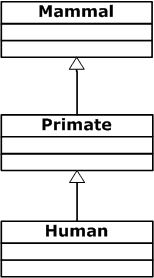
\includegraphics[width=\maxwidth]{images/ref-advanced-topics-refactoring-and-schema-evolution-inheritance-refactoring.png}
\end{center}
In this example you cannot introduce a 'Animal' class above the 'Mammal' or add another class between 'Mammal' and 'Primate'. Also you shouldn't remove an class form the inheritance-hierarchy.

Currently the only possible solution for this refactoring is this.

\begin{enumerate}
\item Create the new hierarchy with different names, preferably in a new package
\item Copy all values from the old classes to the new classes.
\item Redirect all references from existing objects to the new classes.
\end{enumerate}

Take a look at the example to how to add a class into the hierarchy. \hyperref[ref:advanced-topics-refactoring-and-schema-evolution-refactoring-class-hierarchy-inserting-class-into-a-hierarchy]{See "Inserting Class Into A Hierarchy"} (p.~\pageref{ref:advanced-topics-refactoring-and-schema-evolution-refactoring-class-hierarchy-inserting-class-into-a-hierarchy}).

Or how you can remove a class from the inheritance hierarchy. \hyperref[ref:advanced-topics-refactoring-and-schema-evolution-refactoring-class-hierarchy-removing-class-from-a-hierarchy]{See "Removing Class From A Hierarchy"} (p.~\pageref{ref:advanced-topics-refactoring-and-schema-evolution-refactoring-class-hierarchy-removing-class-from-a-hierarchy})

\subsubsection{Removing Class From A Hierarchy}
\label{ref:advanced-topics-refactoring-and-schema-evolution-refactoring-class-hierarchy-removing-class-from-a-hierarchy}

In this example we have a Human class which inherits from the Primate class. Now we want to remove the Primate class and let the Human class inherit directly from the Mammal class.

\begin{center}
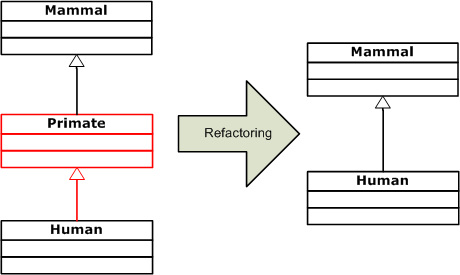
\includegraphics[width=\maxwidth]{images/ref-advanced-topics-refactoring-and-schema-evolution-remove-type-from-hierachy.png}
\end{center}
Unfortunately db4o doesn't support this kind of refactoring. We need to use a work-around. Basically we create a copy of the Human class with the new Inheritance-hierarchy and the copy the existing data over.

\paragraph*{Step by Step}

\begin{enumerate}
\item Create a copy of the Human class, for example HumanNew!
\item Change the inheritance of the HumanNew class to inherit directly from the Mammal class.
\item After that, load all existing Human-instances, copy the values over to HumanNew-instances. Store the HumanNew-instance and delete the old Human-instances
\end{enumerate}

Now the objects have the new inheritance hierarchy. You can delete the old Human class.

\begin{lstlisting}
ObjectSet<Human> allMammals = container.query(Human.class);
for (Human oldHuman : allMammals) {
    HumanNew newHuman = new HumanNew("");
    newHuman.setBodyTemperature(oldHuman.getBodyTemperature());
    newHuman.setIq(oldHuman.getIq());
    newHuman.setName(oldHuman.getName());

    container.store(newHuman);
    container.delete(oldHuman);
}
\end{lstlisting}

{\small\itshape RemoveClassFromHierarchy.java: copy the data from the old type to the new one\par}
\medskip

Note that this example doesn't change existing references from the old instances to the new ones. You need to do this manually as well.

\subsubsection{Inserting Class Into a Hierarchy}
\label{ref:advanced-topics-refactoring-and-schema-evolution-refactoring-class-hierarchy-inserting-class-into-a-hierarchy}

In this example we have a Human class witch inherits from the Mammal class. Now we want to introduce a new Primate class and let the Human class inherit from it.

\begin{center}
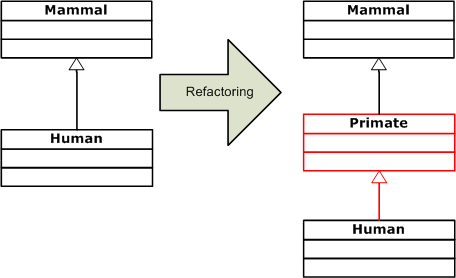
\includegraphics[width=\maxwidth]{images/ref-advanced-topics-refactoring-and-schema-evolution-add-new-type-to-hierachy.png}
\end{center}
Unfortunately db4o doesn't support this kind of refactoring. We need to use a work-around. Basically we create a copy of the Human class with the new Inheritance-hierarchy and the copy the existing data over.

\paragraph*{Step by Step}

\begin{enumerate}
\item Create the new Primate class
\item Create a copy of the Human class, for example HumanNew!
\item Change the HumanNew class to inherit from the new Primate class instead of the Mammal class.
\item After that, load all existing Human-instances, copy the values over to HumanNew instances. Store the HumanNew instance and delete the old Human-instances
\end{enumerate}

Now the objects have the new inheritance hierarchy. You can delete the old Human class.

\begin{lstlisting}
ObjectSet<Human> allMammals = container.query(Human.class);
for (Human oldHuman : allMammals) {
    HumanNew newHuman = new HumanNew("");
    newHuman.setBodyTemperature(oldHuman.getBodyTemperature());
    newHuman.setIq(oldHuman.getIq());
    newHuman.setName(oldHuman.getName());

    container.store(newHuman);
    container.delete(oldHuman);
}
\end{lstlisting}

{\small\itshape AddClassToHierarchy.java: copy the data from the old type to the new one\par}
\medskip

Note that this example doesn't change existing references from the old instances to the new ones. You need to do this manually as well.

\section{Exception Handling}
\label{ref:advanced-topics-exceptions}

A part of the db4o operations is handling possible exceptions. There are two fundamental different exception-types for db4o. The recoverable exceptions and the fatal exceptions.

\subsection*{Recoverable Exceptions}

The recoverable exceptions are all exceptions which don't endanger the consistency of the database. For example if a event callback throws an exception. After a recoverable exception you can continue to work with the object container.

Typical recoverable exceptions are:

\begin{itemize}
\item Exceptions in callbacks.
\item Passing invalid ids to the object container.
\item Unsupported schema-changes.
\item Constraint-violations.
\end{itemize}

\subsection*{Fatal Exceptions}

A fatal exception will immediately shut down the object container without committing anything. This tries to protect the database from damaging itself. Any exception which happens in the db4o core and is not expected and handled is considered as a fatal exception. Because when an exception happens in the db4o-core, it could cause a invalid state in the db4o-core and then cause further errors and lead to database corruption. That's why the policy it the stop immediately any operation after a fatal exception.

Typical fatal recoverable exceptions are:

\begin{itemize}
\item Exceptions related to runtime, like OutOfMemory-exceptions
\item Exceptions related to corrupted database-files.
\end{itemize}

\subsection*{Handle-Exceptions}

Take a look a the list of the most common db4o related exceptions. \hyperref[ref:advanced-topics-exceptions-exception-types]{See "Exception Types"} (p.~\pageref{ref:advanced-topics-exceptions-exception-types}) Handling db4o exceptions is nothing special and complies with regular exception handling.\hyperref[ref:advanced-topics-exceptions-how-to-work-with-db4o-exceptions]{See "How To Work With db4o Exceptions"} (p.~\pageref{ref:advanced-topics-exceptions-how-to-work-with-db4o-exceptions})

\subsection{Exception Types}
\label{ref:advanced-topics-exceptions-exception-types}

Using db4o you will have to deal with db4o-specific exceptions and system exceptions thrown directly out of db4o.

db4o-specific exceptions are unchecked exceptions, which all inherit from a single root class Db4oException.

In Java Unchecked exceptions are inherited from RuntimeExceptions class, while in .NET all exceptions are unchecked.

db4o-exceptions are chained; you can get the cause of the exception using:

Java:

\texttt{db4oException.getCause();}

In order to see all db4o-specific exceptions you can examine the hierarchy of Db4oException class. Currently the following exceptions are available:

\textbf{Db4oException }- db4o exception wrapper: Exceptions occurring during internal processing will be proliferated to the client calling code encapsulated in an exception of this type.

\textbf{BackupInProgressException} - An exception to be thrown when another process is already busy with the backup.

\textbf{ConstraintViolationException }- Base class for all constraint violations.

\textbf{UniqueFieldValueConstraintViolationException} - An exception which will be thrown when the \hyperref[ref:advanced-topics-unique-constraints]{unique constrain} (p.~\pageref{ref:advanced-topics-unique-constraints}) is violated.

\textbf{DatabaseClosedException} - An exception to be thrown when the database was closed or failed to open.

\textbf{DatabaseFileLockedException} - This exception is thrown during any of db4o open calls if the database file is locked by another process.

\textbf{DatabaseMaximumSizeReachedException} - This exception is thrown if the database size is bigger than possible. \hyperref[ref:troubleshoot-increasing-the-maximum-database-file-size]{See "Increasing The Maximum Database File Size"} (p.~\pageref{ref:troubleshoot-increasing-the-maximum-database-file-size})

\textbf{DatabaseReadOnlyException} - This exception is thrown when a write operation was attempted on a database in read-only mode.

\textbf{GlobalOnlyConfigException} - This exception is thrown when you try to change a setting on a open object container, but this setting cannot be changed at runtime.

\textbf{IncompatibleFileFormatException} - An exception to be thrown when an open operation is attempted on a file(database), which format is incompatible with the current version of db4o.

\textbf{InvalidIDException} - an exception to be thrown when an ID format supplied to \#bind or \#getById methods is incorrect.

\textbf{InvalidPasswordException} - This exception is thrown when a client tries to connect to a server with the wrong password.

\textbf{EventException} - This exception is thrown when a exception is thrown in a event callback.

\textbf{OldFormatException} - An exception to be thrown when an old file format was detected and the file could not be open.

\textbf{ReflectException} - An exception to be thrown when a class can not be stored or instantiated by current db4o reflector.

\textbf{ReplicationConflictException} - an exception to be thrown when a conflict occurs and no ReplicationEventListener is specified.

\subsection{How To Work With db4o Exceptions}
\label{ref:advanced-topics-exceptions-how-to-work-with-db4o-exceptions}

Appropriate exception handling will help you to create easy to support systems, saving your time and efforts in the future. The following hints identify important places for exception handling. Take also a look at the list of \hyperref[ref:advanced-topics-exceptions-exception-types]{common db4o exceptions} (p.~\pageref{ref:advanced-topics-exceptions-exception-types}).

\begin{enumerate}
\item Opening a database file can throw a DatabaseFileLockedException.

\begin{lstlisting}
try{
    ObjectContainer container = Db4oEmbedded.openFile("database.db4o");
} catch (DatabaseFileLockedException e){
    // Database is already open!
    // Use another database-file or handle this case gracefully
}
\end{lstlisting}

{\small\itshape ImportantExceptionCases.java: If the database is already open\par}
\medskip
\item Opening a client connection can throw IOException.

\begin{lstlisting}
try{
    final ObjectContainer container = Db4oClientServer.openClient("localhost", 1337, "sa", "sa");

} catch(Db4oIOException e){
    // Couldn't connect to the server.
    // Ask for new connection-settings or handle this case gracefully
}
\end{lstlisting}

{\small\itshape ImportantExceptionCases.java: Cannot connect to the server\par}
\medskip
\item Working with \hyperref[ref:advanced-topics-unique-constraints]{db4o-unique constraints} (p.~\pageref{ref:advanced-topics-unique-constraints}) the commit may throw exceptions when the constraints are violated.

\begin{lstlisting}
container.store(new UniqueId(42));
container.store(new UniqueId(42));
try{
    container.commit();
} catch (UniqueFieldValueConstraintViolationException e){
    // Violated the unique-constraint!
    // Retry with a new value or handle this gracefully
    container.rollback();
}
\end{lstlisting}

{\small\itshape ImportantExceptionCases.java: Violation of the unique constraint\par}
\medskip
\end{enumerate}

\section{db4o Reflection API}
\label{ref:advanced-topics-db4o-reflection-api}

Reflection gives your code access to internal information for classes loaded into the JVM. It allows you to explore the structure of objects at runtime. In the case of reflection metadata is the description of classes and objects within the JVM, including their fields, methods and constructors. It allows the programmer to select target classes at runtime, create new objects, call their methods and operate with the fields.

In order to persist object db4o uses the reflection to read object and store their values. You can exchange this reflector layer in the \hyperref[ref:configuration-common-reflector]{configuration} (p.~\pageref{ref:configuration-common-reflector}).

By default the JdkReflector is used. This reflector also allows you to specify the right class-loader.

\begin{lstlisting}
EmbeddedConfiguration configuration = Db4oEmbedded.newConfiguration();
configuration.common().reflectWith(
        new JdkReflector(Thread.currentThread().getContextClassLoader()));
\end{lstlisting}

{\small\itshape CommonConfigurationExamples.java: Change the reflector\par}
\medskip

It's also possible to use very special class resolving strategy by implementing the JdkLoader-interface. For example when you want to look up classes in multiple class loaders.

\begin{lstlisting}
EmbeddedConfiguration configuration = Db4oEmbedded.newConfiguration();

JdkLoader classLookUp = new ClassLoaderLookup(
        Thread.currentThread().getContextClassLoader(),
        new URLClassLoader(new URL[]{new URL("file://./some/other/location")}));
configuration.common().reflectWith(new JdkReflector(classLookUp));

ObjectContainer container = Db4oEmbedded.openFile("database.db4o");
\end{lstlisting}

{\small\itshape CommonConfigurationExamples.java: Complex class loader scenario\par}
\medskip

\begin{lstlisting}
public class ClassLoaderLookup implements JdkLoader {
    private final List<ClassLoader> classLoaders;

    ClassLoaderLookup(ClassLoader...classLoaders) {
        this.classLoaders = Arrays.asList(classLoaders);
    }

    ClassLoaderLookup(Collection<ClassLoader> classLoaders) {
        this.classLoaders = new ArrayList<ClassLoader>(classLoaders);
    }

    @Override
    public Class loadClass(String className) {
        for (ClassLoader loader : classLoaders) {
            Class<?> theClass = null;
            try {
                theClass = loader.loadClass(className);
                return theClass;
            } catch (ClassNotFoundException e) {
                // first check the other loaders
            }
        }
        throw new RuntimeException(new ClassNotFoundException(className));
    }

    @Override
    public Object deepClone(Object o) {
        return new ClassLoaderLookup(classLoaders);
    }
}
\end{lstlisting}

{\small\itshape ClassLoaderLookup.java: Complex class loader scenario\par}
\medskip

If you need some special treatment you can create you're own reflector implementation. \hyperref[ref:advanced-topics-db4o-reflection-api-creating-your-own-reflector]{See "Creating your own reflector"} (p.~\pageref{ref:advanced-topics-db4o-reflection-api-creating-your-own-reflector})

db4o has also a generic reflector which can deal with stored objects without using the original class. \hyperref[ref:advanced-topics-db4o-reflection-api-genericreflector]{See "GenericReflector"} (p.~\pageref{ref:advanced-topics-db4o-reflection-api-genericreflector})

\subsection{Creating your own reflector}
\label{ref:advanced-topics-db4o-reflection-api-creating-your-own-reflector}

By default db4o uses the JdkReflector . As alternative you can create your own reflector and use it with db4o. In order to do so you need to implement the Reflector interface. And then pass an instance of your implementation to db4o.

Here's an example of a logging reflector. Its only difference from standard reflector is that information about loaded classes is outputted to console:

\begin{lstlisting}
class LoggerReflector implements Reflector{
    private final Reflector readReflector;

    public LoggerReflector() {
        this(new JdkReflector(Thread.currentThread().getContextClassLoader()));
    }

    public LoggerReflector(Reflector readReflector) {
        this.readReflector = readReflector;
    }

    @Override
    public void configuration(ReflectorConfiguration reflectorConfiguration) {
        readReflector.configuration(reflectorConfiguration);
    }

    @Override
    public ReflectArray array() {
        return readReflector.array();
    }

    @Override
    public ReflectClass forClass(Class aClass) {
        System.out.println("Reflector.forClass("+aClass+")");
        return readReflector.forClass(aClass);
    }

    @Override
    public ReflectClass forName(String className) {
        System.out.println("Reflector.forName("+className+")");
        return readReflector.forName(className);
    }

    @Override
    public ReflectClass forObject(Object o) {
        System.out.println("Reflector.forObject("+o+")");
        return readReflector.forObject(o);
    }

    @Override
    public boolean isCollection(ReflectClass reflectClass) {
        return readReflector.isCollection(reflectClass);
    }

    @Override
    public void setParent(Reflector reflector) {
        readReflector.setParent(reflector);
    }

    @Override
    public Object deepClone(Object o) {
        return new LoggerReflector((Reflector) readReflector.deepClone(o));
    }
}
\end{lstlisting}

{\small\itshape ReflectorExamples.java: Logging reflector\par}
\medskip

\subsection{GenericReflector}
\label{ref:advanced-topics-db4o-reflection-api-genericreflector}

db4o uses reflection internally for persisting and instantiating user objects. Reflection helps db4o to manage classes in a general way while saving. It also makes instantiation of objects using class name possible. However db4o reflection API can also work on generic objects when a class information is not available.

db4o uses a generic reflector as a decorator around specific reflector. The generic reflector is set when an object container is opened. All subsequent reflector calls are routed through this decorator.

The generic reflector keeps list of known classes in memory. When the generic reflector is called, it first checks its list of known classes. If the class cannot be found, the task is transferred to the delegate reflector. If the delegate fails as well, generic objects are created, which hold simulated "field values" in an array of objects.

Generic reflector makes possible the following use cases:

\begin{itemize}
\item Running a db4o server without deploying application classes.
\item Easier access to stored objects where classes or fields are not available.
\item Building interfaces to db4o from any programming language.
\end{itemize}

One of the live use cases is the ObjectManager, which uses the generic reflector to read C\# objects from Java.

The generic reflector is automatically used when the class of a stored object is not found.

\section{Runtime Statistics}
\label{ref:advanced-topics-runtime-statistics}

The db4o runtime statistics is a monitoring feature allowing to collect various important runtime data. This data can be crucial in resolving performance issues, analyzing usage patterns, predicting resource bottlenecks etc. Runtime Statistics can be collected both in the application testing stage and in an application deployed to production system. In the first case this data can help to estimate hardware requirements and analyze the stability of the system. In the latter case, the data can be used to fine-tune performance, find problems and fix bugs. Take a look how you install the statistics and monitor them.

\subsection*{Install And Monitor}

On the Java platform all runtime statistics are published through the JMX interface. This means that you can use any JMX client to monitor the statistics. \hyperref[ref:advanced-topics-runtime-statistics-install-and-monitor]{See "Install and Monitor"} (p.~\pageref{ref:advanced-topics-runtime-statistics-install-and-monitor})

\subsection*{Available Statistics}

Currently following statistics are available.

\begin{itemize}
\item \hyperref[ref:advanced-topics-runtime-statistics-monitor-queries]{Query Monitoring} (p.~\pageref{ref:advanced-topics-runtime-statistics-monitor-queries}): Monitor how queries behave and perform.
\item \hyperref[ref:advanced-topics-runtime-statistics-monitor-object-lifecycle]{Object Lifecycle Monitoring} (p.~\pageref{ref:advanced-topics-runtime-statistics-monitor-object-lifecycle}): Monitor how many objects are stored, deleted and activated.
\item \hyperref[ref:advanced-topics-runtime-statistics-monitor-io]{IO Monitoring} (p.~\pageref{ref:advanced-topics-runtime-statistics-monitor-io}): Monitor the IO-operations of db4o.
\item \hyperref[ref:advanced-topics-runtime-statistics-monitor-network]{Network Monitoring} (p.~\pageref{ref:advanced-topics-runtime-statistics-monitor-network}): Monitor the network operations of db4o.
\item \hyperref[ref:advanced-topics-runtime-statistics-monitor-reference-system]{Reference System Monitoring} (p.~\pageref{ref:advanced-topics-runtime-statistics-monitor-reference-system}): Monitor db4o's reference system.
\end{itemize}

\subsection{Install and Monitor}
\label{ref:advanced-topics-runtime-statistics-install-and-monitor}

On the Java platform all runtime statistics are published through the JMX interface. This means that you can use any JMX client to monitor the statistics.

\subsubsection*{Installing the Monitoring Support}

The first thing we need to do is to add the monitoring support to the db4o configuration. The monitoring-support are in \hyperref[ref:dependency-overview]{the optional-jar s} (p.~\pageref{ref:dependency-overview}). So you need to add those for the monitoring support.

Monitoring adds a small overhead to the regular db4o operations. Therefore the monitoring support is distributed across different monitoring options, so that you can add only the options you need.

Currently following options are available:

\begin{itemize}
\item \hyperref[ref:advanced-topics-runtime-statistics-monitor-queries]{Query Monitoring} (p.~\pageref{ref:advanced-topics-runtime-statistics-monitor-queries}): Monitor how queries behave and perform.
\item \hyperref[ref:advanced-topics-runtime-statistics-monitor-object-lifecycle]{Object Lifecycle Monitoring} (p.~\pageref{ref:advanced-topics-runtime-statistics-monitor-object-lifecycle}): Monitor how many objects are stored, deleted and activated.
\item \hyperref[ref:advanced-topics-runtime-statistics-monitor-io]{IO Monitoring} (p.~\pageref{ref:advanced-topics-runtime-statistics-monitor-io}): Monitor the IO-operations of db4o.
\item \hyperref[ref:advanced-topics-runtime-statistics-monitor-network]{Network Monitoring} (p.~\pageref{ref:advanced-topics-runtime-statistics-monitor-network}): Monitor the network operations of db4o.
\item \hyperref[ref:advanced-topics-runtime-statistics-monitor-reference-system]{Reference System Monitoring} (p.~\pageref{ref:advanced-topics-runtime-statistics-monitor-reference-system}): Monitor db4o's reference system.
\end{itemize}

\subsubsection*{Monitor With JConsole}

As said, the statistics are published through the JMX-interface (Java Management Extensions). Therefore you can use any JMX-client to monitor db4o. The JDK brings its own JMX-client with it: The \href{http://java.sun.com/javase/6/docs/technotes/guides/visualvm/intro.html}{JConsole}-application is located in the bin-folder of the JDK-installation. Start the JConsole and connect your running db4o application. Then you will find the db4o related readings on the "MBeans" tab. In the treeview on the left, you will see "com.db4o.monitoring".

Below this tree node you will find all open ObjectContainers that have JMX monitoring enabled. For each of them the respective runtime statistics categories will be listed. If you select the "Attributes" node for any of them, the corresponding set of attribute values will be shown along with their most recent reading.

By double clicking on the number value a graph will be displayed.

Some Monitoring-Nodes also provide notifications. You can subscribe to this notifications. In the categories where the "Notifications" node is visible, you can select it and click "Subscribe" on the bottom right. For example we provide notifications about unoptimized native queries and about class index scans.

\begin{center}
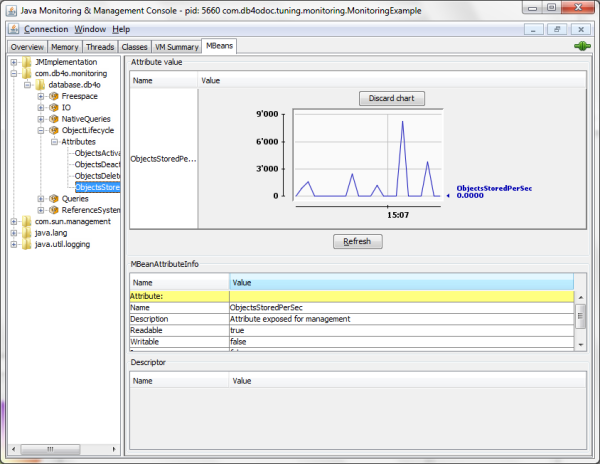
\includegraphics[width=\maxwidth]{images/ref-advanced-topics-runtime-statistics-jconsole.png}
\end{center}
\subsection{Monitoring Queries}
\label{ref:advanced-topics-runtime-statistics-monitor-queries}

You can monitor queries to find out more about the runtime behavior of your application.

\subsubsection*{Configure the Query Monitoring Support}

First you need to add the monitoring support to the db4o configuration. There are two separate items. The QueryMonitoringSupport will monitor the very basic query operations. The NativeQueryMonitoringSupport adds additional statistics about  native queries.

\begin{lstlisting}
configuration.common().add(new QueryMonitoringSupport());
configuration.common().add(new NativeQueryMonitoringSupport());
\end{lstlisting}

{\small\itshape QueryMonitoring.java: Add query monitoring\par}
\medskip

\subsubsection*{The Query Statistics}

\textbf{AverageQueryExecutionTime} : Tells you how long on average a query takes to execute. Of course this heavily depends on the complexity of the queries. However if this number is high, you maybe should improve you query-performance. For example by adding additional indexes. \hyperref[ref:basics-indexing]{See "Indexing"} (p.~\pageref{ref:basics-indexing})

\textbf{ClassIndexScansPerSecond}: Tells you the number of queries which required to scan through all objects. This means that a query couldn't use a field index and therefore required to go through all objects. This is of course slow. You should try to keep this number low by adding the right indexes on fields. \hyperref[ref:basics-indexing]{See "Indexing"} (p.~\pageref{ref:basics-indexing})

\textbf{QueriesPerSecond}: Tells you how many queries run per second.

\textbf{Loaded From Class Index Notifications}: The query statistics can notify you every time a query used the class-index and couldn't utilize a field index. You should try to avoid loading by class index by adding the right indexes on fields. \hyperref[ref:basics-indexing]{See "Indexing"} (p.~\pageref{ref:basics-indexing})

\subsubsection*{The Native Query Statistics}

\textbf{NativeQueriesPerSecond}: Tells you how many native queries per second run.

\textbf{UnoptimizedNativeQueriesPerSecond}: Tells you how many unoptimized native queries run per second. Such queries need to instantiate all objects which is a slow operation. If this number is high, you should try to simplify your queries.

\textbf{Native Query Not Optimized Notifications}: The native query statistics can notify you every time a query couldn't be optimized. You should try to avoid such queries. Try to simplify the native query or fall back to SODA-queries.

\subsection{Monitor Object Lifecycle}
\label{ref:advanced-topics-runtime-statistics-monitor-object-lifecycle}

You can monitor the object lifecycle statistics of db4o to find out more about the runtime behavior of your application.

\subsubsection*{Configure the Object Lifecycle Monitoring Support}

In order to monitor the object lifecycle statistics, you need to add the monitoring support to the configuration.

\begin{lstlisting}
configuration.common().add(new ObjectLifecycleMonitoringSupport());
\end{lstlisting}

{\small\itshape ObjectLifecycleMonitoring.java: Monitor the object lifecycle statistics\par}
\medskip

\subsubsection*{The Object Lifecycle Statistics}

\textbf{ObjectsActivatedPerSec}: Tells you how many objects are \hyperref[ref:basics-activation]{activated} (p.~\pageref{ref:basics-activation}) per second. Activation can consume a lot of time for complex object graphs. If there's a lot of time spend with activating objects, you may want to reduce the amount of activated objects. One of the best way to activate only the minimum set of objects is to use \hyperref[ref:basics-activation-concept-transparent-activation-framework]{transparent activation} (p.~\pageref{ref:basics-activation-concept-transparent-activation-framework}).

\textbf{ObjectsDeactivatedPerSec}: Tells you how many objects are deactivate per second.

\textbf{ObjectsDeletedPerSec}: Tells you how many objects are deleted per second.

\textbf{ObjectsStoredPerSec}: Tells you how many objects are stored per second.

\subsection{Monitor IO}
\label{ref:advanced-topics-runtime-statistics-monitor-io}

You can monitor the IO-operations of db4o to find out more about the runtime behavior of your application.

\subsubsection*{Configure the IO Monitoring Support}

In order to monitor the IO activities of db4o you need to configure the IO monitoring support.

\begin{lstlisting}
configuration.common().add(new IOMonitoringSupport());
\end{lstlisting}

{\small\itshape IOMonitoring.java: Add IO-Monitoring\par}
\medskip

\subsubsection*{The IO Statistics}

\textbf{BytesReadPerSecond}: Tells you how many bytes are read per second from the disk.

\textbf{BytesWrittenPerSecond}: Tells you how many bytes are written to disk per second.

\textbf{ReadsPerSecond}: Tells how many read requests are issues per second.

\textbf{SyncsPerSecond}: Tells you how many sync-operations are done per second. The sync-operation is a part of the commit-process. I forces the runtime and operating system to flush all buffers to the disk to ensure that the data are safely stored. The sync operation is normally a costly operation, since it need to wait on the physical disk to finish all write operations

.\textbf{WritesPerSecond}: Tells you how may write requests are issued per second.

\subsection{Monitor Freespace}
\label{ref:advanced-topics-runtime-statistics-monitor-freespace}

You can monitor the freespace-manager to find out more about the runtime behavior of your application.

\subsubsection*{Configure the Freespace Monitoring Support}

To monitor the freespace manager you need to add the monitoring support to the db4o configuration.

\begin{lstlisting}
configuration.common().add(new FreespaceMonitoringSupport());
\end{lstlisting}

{\small\itshape FreespaceMonitoring.java: Monitor the free-space system\par}
\medskip

\subsubsection*{The Freespace Statistics}

\textbf{AverageSlotSize}: Tells you how big the average slot is. When you store larger objects, they need larger slots to fit it.

\textbf{ReusedSlotsPerSecond}: Tells you how many slots can be reused. When an object is deleted or modified, its old slot is released and can be reused. If you modify and delete a lot of objects, but the slots cannot be reused, then the database-file will fragment.

When this number is low but the free-space increases and increases then you have a fragmentation issue. \hyperref[ref:advanced-topics-defragment]{Defragment} (p.~\pageref{ref:advanced-topics-defragment}) your database. Use the \hyperref[ref:configuration-id-system]{btree-id-system.} (p.~\pageref{ref:configuration-id-system})

\textbf{SlotCount}: Tells you how many slots are used by the database. As more and more objects are stored, the slot count will increase.

\textbf{TotalFreespace}: Tells you how much freespace there is in the database-file.A hight free-space number with a low reused slots number indicates database fragmentation. \hyperref[ref:advanced-topics-defragment]{Defragment} (p.~\pageref{ref:advanced-topics-defragment}) your database. Use the \hyperref[ref:configuration-id-system]{btree-id-system.} (p.~\pageref{ref:configuration-id-system})

\subsection{Monitor Network}
\label{ref:advanced-topics-runtime-statistics-monitor-network}

You can monitor the network-operations of db4o in client-server mode.

\subsubsection*{Configure the Network Monitoring Support}

First you need to add the monitoring support to the db4o configuration. The network monitoring support is in two separate configuration-items. The NetworkingMonitoringSupport can be used on the server and client to monitor the network statistics.

\begin{lstlisting}
configuration.common().add(new NetworkingMonitoringSupport());
\end{lstlisting}

{\small\itshape CSMonitoring.java: Add the network monitoring support\par}
\medskip

The ClientConnectionsMonitoringSupport can be added to the db4o server to monitor the connected clients.

\begin{lstlisting}
configuration.addConfigurationItem(new ClientConnectionsMonitoringSupport());
\end{lstlisting}

{\small\itshape CSMonitoring.java: Add the client connections monitoring support\par}
\medskip

\subsubsection*{The Network Statistics}

\textbf{BytesReceivedPerSecond}: Tells you how many bytes this client or server has receives per second.

\textbf{BytesSentPerSecond}: Tells you how many bytes this client or server sends per second.

\textbf{MessagesSentPerSecond}: Tells you how many messages this client or server sends per second.

\textbf{ConnectedClientCount}: Tells you how many clients are connected to this server.

\subsection{Monitor Reference System}
\label{ref:advanced-topics-runtime-statistics-monitor-reference-system}

You can monitor the \hyperref[ref:basics-indentity-concept-reference-cache]{reference-system} (p.~\pageref{ref:basics-indentity-concept-reference-cache}) to find out more about the runtime behavior of your application. The reference-system ensures that each object has only one in memory representation.

\subsubsection*{Configure the Reference System Monitoring Support}

First you need to add the monitoring support to the db4o configuration.

\begin{lstlisting}
configuration.common().add(new ReferenceSystemMonitoringSupport());
\end{lstlisting}

{\small\itshape ReferenceSystemMonitoring.java: Add reference system monitoring\par}
\medskip

\subsubsection*{The Freespace Statistics}

\textbf{ObjectReferenceCount}: Tells you how many references are currently hold in the reference-system. By default db4o uses weak references to objects. If this count is very high, you might hold unnecessary references to persisted objects in your application.

\section{Diagnostics}
\label{ref:advanced-topics-diagnostics}

The db4o engine provides user with a special mechanism showing runtime diagnostics information. Diagnostics can be switched on in the configuration before opening the database file:

The DiagnosticListener is a callback interface tracking diagnostic messages from different parts of the system.

\begin{lstlisting}
EmbeddedConfiguration configuration = Db4oEmbedded.newConfiguration();
configuration.common().diagnostic().addListener(new DiagnosticToConsole());
\end{lstlisting}

{\small\itshape CommonConfigurationExamples.java: Add a diagnostic listener\par}
\medskip

\subsection*{Built-in Listeners}

There are two build in listeners, which print the output to the console

\begin{itemize}
\item DiagnosticToConsole:Prints diagnostic messages to the console.
\item DiagnosticToTrace: Only on .NET, prints diagnostic messages to the debug output window.
\end{itemize}

\subsection*{Messages-Types}

Every diagnostic message is represented by it's own type. You can filter the messages by checking for certain instances. Take a look how you can filter for \hyperref[ref:advanced-topics-diagnostics-diagnostic-messages-filter]{certain messages.} (p.~\pageref{ref:advanced-topics-diagnostics-diagnostic-messages-filter})

\begin{itemize}
\item \textbf{MissingClass}: Notifies you that a class couldn't be found. You should add that class in order to avoid problems. If you've renamed the class, you \hyperref[ref:advanced-topics-refactoring-and-schema-evolution]{should rename} (p.~\pageref{ref:advanced-topics-refactoring-and-schema-evolution}) it in the database or add \hyperref[ref:configuration-common-alias]{an alias} (p.~\pageref{ref:configuration-common-alias}).
\item \textbf{DefragmentRecommendation}: Notifies you that you should consider to \hyperref[ref:advanced-topics-defragment]{defragment} (p.~\pageref{ref:advanced-topics-defragment}) the database.
\item \textbf{LoadedFromClassIndex}: Notifies you that db4o couldn't use a field-index to perform a query. This means that the query runs extremely slow on larger data sets. Consider adding a \hyperref[ref:basics-indexing]{field-index} (p.~\pageref{ref:basics-indexing}).
\item \textbf{DescendIntoTranslator}: Means that you a query couldn't be optimized, because the query touches a class \hyperref[ref:advanced-topics-type-handling-translators]{with a translator} (p.~\pageref{ref:advanced-topics-type-handling-translators}). Therefore the query runs slow. You should consider working without a translator or changing the query.
\item \textbf{ClassHasNoFields}: You stored a class which has no fields. Even when the class has no fields it need to maintain its class index and needs to be stored. So it adds overhead for storing 'empty' objects. You should consider removing the empty class.
\item \textbf{DeletionFailed}: db4o failed to delete a object from the database.
\item \textbf{UpdateDepthGreaterOne}: You have configured a update depth greater one. A large update depth slows down updates significantly. Consider reducing the update-depth and use another strategies to update objects correctly, like \hyperref[ref:basics-update-concept-transparent-persistence]{transparent persistence} (p.~\pageref{ref:basics-update-concept-transparent-persistence}).
\item \textbf{NativeQueryNotOptimized}: A native query couldn't be optimized. An unoptimized query runs significantly slower than a optimized query. Consider to simplify you're query.
\item \textbf{NativeQueryOptimizerNotLoaded}: Couldn't load the native query optimizer. Ensure that all required jar are added to your application.
\item \textbf{NotTransparentActivationEnabled}: Notifies you when a class doesn't support transparent activation. Such object need to be fully activated and slow down the activation process.
\item \textbf{ObjectFieldDoesNotExist}: A query uses a object-field which doesn't exist. Check you're queries to use only exising fields.
\end{itemize}

\subsection{Diagnostic Messages Filter}
\label{ref:advanced-topics-diagnostics-diagnostic-messages-filter}

The standard listeners can potentially produce quite a lot of messages. By writing your own DiagnosticListener you can filter that information.

On the stage of application tuning you can be interested in optimizing performance through indexing. Diagnostics can help you with giving information about queries that are running on un-indexed fields. By having this information you can decide which queries are frequent and heavy and should be indexed, and which have little performance impact and do not need an index. Field indexes dramatically improve query performance but they may considerably reduce storage and update performance.

In order to get rid of all unnecessary diagnostic information and concentrate on indexes let's create special diagnostic listener:

\begin{lstlisting}
private static class DiagnosticFilter implements DiagnosticListener{
    private final Set<Class> filterFor;
    private final DiagnosticListener delegate;

    private DiagnosticFilter(DiagnosticListener delegate,Class<? extends Diagnostic>...filterFor) {
        this.delegate = delegate;
        this.filterFor = new HashSet<Class>(Arrays.asList(filterFor));
    }

    public void onDiagnostic(Diagnostic diagnostic) {
        Class<?> type = diagnostic.getClass();
        if(filterFor.contains(type)){
            delegate.onDiagnostic(diagnostic);
        }
    }
}
\end{lstlisting}

{\small\itshape DiagnosticsExamples.java: A simple message filter\par}
\medskip

After that we can use the filter-listener. It takes two arguments. The first one is a regular listener, the second is a list of all messages which are passed through.

\begin{lstlisting}
EmbeddedConfiguration configuration = Db4oEmbedded.newConfiguration();
configuration.common().diagnostic()
        .addListener(new DiagnosticFilter(new DiagnosticToConsole(), LoadedFromClassIndex.class));
\end{lstlisting}

{\small\itshape DiagnosticsExamples.java: Filter for unindexed fields\par}
\medskip

